%_______________________________________________________________________________
%class
%_______________________________________________________________________________
%\documentclass[a4paper,11pt,onecolumn,final,german,openbib]{scrbook}
\documentclass[a4paper,11pt,oneside,final,english,toc=bib,draft]{scrbook}

% fonts

\usepackage{fontspec}
\setmainfont{Libre Baskerville} % Libre Baskerville - Palatino Linotype - Constantia
\setsansfont{Helvetica} % Arial
\setmonofont{Consolas} % Hack

\usepackage[OT1]{eulervm}
% \usepackage{mathdesign}

%_______________________________________________________________________________
% page borders
%_______________________________________________________________________________
\addtolength{\headheight}{2cm}
%\addtolength{\topmargin}{2cm}
\setlength{\oddsidemargin}{1.0cm}
\setlength{\evensidemargin}{0.5cm}
\setlength{\textwidth}{14.3cm}
\setlength{\parindent}{0mm}

%_______________________________________________________________________________
% packages
%_______________________________________________________________________________
% \usepackage{german}
\usepackage{babel}[uk-english] % english hyphenation
% \usepackage{textcomp}
\usepackage{csquotes} % defines \enquote for enquoting text

\usepackage{mathtools} % defines common math symbols and tools
\usepackage{amssymb,amsfonts} % more math symbols and fonts
\usepackage{physics} % all-purpose physics and math notation
\usepackage[separate-uncertainty=true,per-mode=power,group-separator={,}]{siunitx} % numbers with units
% \usepackage[version=4]{mhchem} % chemical equations
% \usepackage{dsfont} % math font for double-stroked letters
% \usepackage{slashed} % math font for slashed symbols

\usepackage{graphicx} % \includegraphics and \textcolor
\usepackage{xcolor} % define common colors
% \usepackage{subfigure}
\usepackage{float} % 
\usepackage{caption} % configure caption style for figures and tables
\usepackage{subcaption} % subfigures
\usepackage{placeins} % defines \FloatBarrier, which forces floats to be rendered before
\usepackage{enumitem} % better lists

% \usepackage{url}
% \usepackage{enumerate}

\usepackage{booktabs} % prettier tables
% \usepackage{multirow}

% \usepackage{appendix} % appendix section

\usepackage{todonotes} % insert TODO notes

\usepackage[style=ieee]{biblatex} % ,sorting=none style=h-physrev3 defernumbers=true
\bibliography{thesis}


\graphicspath{ {./images/} }

\usepackage[draft=false]{hyperref} % links inside document
\hypersetup{
  colorlinks=true,
  linkcolor=blue,
  citecolor=teal
}

\captionsetup[figure]{labelfont=bf,format=plain,labelsep=newline} % ,labelsep=period ,margin=1cm
\captionsetup[table]{labelfont=bf,format=plain,labelsep=newline} % ,labelsep=period ,margin=1cm ,labelsep=newline

\renewcommand{\arraystretch}{1.2} % make distance between table rows a bit bigger

\newcommand{\figwidth}{12cm} % default width for all figures

\parindent10mm

% \makesavenoteenv{table}

\usepackage{mgscience}

%_______________________________________________________________________________
% bold fonts for headings
%_______________________________________________________________________________
\font\afont=cmssbx10 scaled \magstep5     % for the title
\font\bfont=cmssbx10 scaled \magstep4     % for chapter headings
\font\cfont=cmssbx10 scaled \magstep3
\font\dfont=cmssbx10 scaled \magstep2     % for section headings and author name
\font\efont=cmssbx10 scaled \magstephalf

%_______________________________________________________________________________
% index depth
%_______________________________________________________________________________
\setcounter{secnumdepth}{3}
\setcounter{tocdepth}{3}

%_______________________________________________________________________________
% new commands
%_______________________________________________________________________________
% \newcommand{\demi}{\frac{1}{2}}

%_______________________________________________________________________________
% renewed commands
%_______________________________________________________________________________
% \renewcommand{\topfraction}{1.}       % this is important for figure placement
% \renewcommand{\bottomfraction}{1.}
\makeatletter
\renewcommand\paragraph{\@startsection{paragraph}{4}{\z@}%
  {-3.25ex\@plus -1ex \@minus -.2ex}%
  {1.5ex \@plus .2ex}%
  {\normalfont\normalsize\bfseries}
}
\makeatother

%_______________________________________________________________________________
% special words, hyphenation
%_______________________________________________________________________________
% \hyphenation{Ba-che-lor-ar-beit}

\pagestyle{empty}
\pagestyle{headings}
%for changing the style on a specific page use \thispagestyle{e.g., empty}

%_______________________________________________________________________________
%_______________________________________________________________________________
\begin{document}
\pagenumbering{roman}

%_______________________________________________________________________________
\begin{titlepage}
  \vspace*{6mm}
  \begin{center}
     {\afont Comparison of 3-dimensional chromatin structures based on single cell Hi-C data}
     \\[3.5cm]
     {\large von}
     \\[3.5cm]
     {\dfont Moritz Gmeiner}
     \\[1.5cm]
     {\dfont Supervisor: PD Dr. Peter Virnau}
     \\[2cm]
     % {\large Bachelorarbeit in Physik \/\\
     %    vorgelegt dem Fachbereich Physik, Mathematik und Informatik (FB 08) \/\\
     %    der Johannes Gutenberg-Universität Mainz \/\\
     %    am 1. April 2012}
     {\large Bachelor Thesis in Physics \/\\
        presented to the faculty physics, mathematics, and computer science (FB 08) \/\\
        of the Johannes Gutenberg University Mainz \/\\
        \today}
   \end{center}
   \vfill
   1. Reviewer: PD Dr. Peter Virnau \\	
   2. Reviewer: Prof. Dr. Friederike Schmid \\
   \vfill
\end{titlepage}

\thispagestyle{empty}
Ich versichere, dass ich die Arbeit selbstständig verfasst und keine 
anderen als die angegebenen Quellen und Hilfsmittel benutzt sowie 
Zitate kenntlich gemacht habe.
\\
\\[3.5cm] 
Mainz, den \today
\vfill
\noindent 
Moritz Gmeiner\\
KOMET\\
Institut für Physik\\
Staudingerweg 7\\
Johannes Gutenberg-Universität
D-55099 Mainz\\
{ \texttt{mgmeiner@students.uni-mainz.de} }

%_______________________________________________________________________________
% \renewcommand\contentsname{Inhaltsverzeichnis}
% \renewcommand\figurename{Abbildung}
% \renewcommand\tablename{Tabelle}

\tableofcontents
\clearpage

\mainmatter
\sloppy

%_______________________________________________________________________________
% \include{...}
\chapter{Introduction} % (fold)
\label{cha:introduction}

\section{DNA and the genome} % (fold)
\label{sec:dna_and_genome}

DNA is the most important long-term information storage \textcolor{orange}{in biology}. It is so fundamental that it is a shared part of all known life, and even some non-living things like viruses\footnote{The question whether or not viruses are alive or not is somewhat dependent on the definition of life and has not been finally decided (and probably never will), but here they shall be considered non-living.}. In eukaryotes, most of the genome\footnote{The term \enquote{genome} typically includes all of the DNA in the cell, including e.g. mitochondrial and plastid DNA. For simplicity, in this work the genome shall include only the DNA in the nucleus, as it is the main and for this work only relevant part} is stored away in the cell's nucleus, a specialised compartment that is separated from the rest of the cell by the nuclear envelope. It is split up into multiple chromosomes, linear, i.e. non-circular, chains of DNA of varying length., the number of which is dependent on the particular species, for example humans have 23 chromosomes while mice, the primary subject of this work, have 20. Different species and cell types also vary in the number of copies of each chromosome they carry: haploid cells for example carry only a single copy of each chromosomes, while diploid cells have two copies of each chromosomes. To fit into the nucleus, the genome needs to be highly packaged: the length of the human genome for example is about \(\SI{2}{\metre}\), while the cell nucleus is merely \(5\)-\(8\) \(\si{\micro\metre}\) in diameter. This packaging occurs at different levels, like histones and the 30-nm fibre. This process of DNA packaging is a very important research topic, as it is involved in transcription initiation, the first step of making proteins from DNA information. \textcolor{orange}{By making certain regions of DNA more or less accessible, specific parts of the genome can either be activated or silenced, which is an important way to regulate gene expression}.

\cite{uzman_essential_2010}

\section{Hi-C} % (fold)
\label{sec:hi_c}

Hi-C is a method of determining the three-dimensional structure of an entire genome utilising a combination of proximity-based ligation and DNA deep sequencing. It is a continuation of a number of previous chromosome conformation capture methods (3C, 4C, 5C) with the goal of moving from targeting specific genetic loci go obtaining a genome-wide map of interactions.

First, the DNA is cross-linked using formaldehyde, making connections between two strands of DNA that are in close proximity. The DNA is then digested by a restriction endonuclease that leaves a 5' staggered end which is filled with biotin-marked residues and ligated under conditions that favour ligation of those cross-linked DNA fragments. The DNA is sheared and selected for the biotin-marked cross-linked DNA fragments. These fragments are then deep sequenced and mapped back onto the genome, giving a list of contacts between positions on the genome.\cite{lieberman-aiden_comprehensive_2009}.

% section hi_c (end)

% section dna_and_genome (end)

% \section{Mathematical Tools} % (fold)
% \label{sec:mathematical_tools}

% \subsection{RMSD} % (fold)
% \label{sec:rmsd}

% The root-mean-square deviation (RMSD) is a mathematical tools for comparing how similar two ordered sets of 3-dimensional points of equal length are and is given for the two sets \( \set{x_i} \) and \( \set{y_i} \) by the formula

% \[
%   \text{RMSD} = \sqrt{ \frac{n} \sum_i \norm{x_i - y_i}^2 }
% \]

% While there are certain ready-made tools to calculate RMSDs of trajectories, for example in VMD's\cite{humphrey_vmd_1996} RMSD Trajectory tool, for this work a more custom approach was chosen in order to have more flexibility. The code for RMSD calculation can be found in the \verb|tools/rmsd.py| file, in particular in the \verb|rmsd(pos1, pos2| function, which calculates the RMSD between two point sets using scipy's\cite{virtanen_scipy_2020} \verb|scipy.spatial.procrustes| function.

% % section rmsd (end)

% section mathematical_tools (end)



%_______________________________________________________________________________
% \chapter{Main Part}

% Die typische Gliederung einer Bachelorarbeit könnte so aussehen, 
% wie im folgenden dargestellt. 
% \medskip

% Verwenden Sie aussagekräftige Kapitelüberschriften, also zum 
% Beispiel {\em Aufbau eines Teilchenbeschleunigers} statt 
% {\em Versuchsaufbau}.


% chapter introduction (end)

%_______________________________________________________________________________


%!TEX root = ../thesis

\chapter{Simulation} % (fold)
\label{cha:simulation}

\section{Model and Simulation Protocol} % (fold)
\label{sec:model_and_simulation_protocol}

The simulation protocol for the entire genome simulations was mostly carried over from (Wettermann et al.\cite{wettermann_minimal_2020}). Additionally simulations of single chromosomes were carried out; the protocol for these simulations is identical to that of the entire genome, except only the beads of the chromosome in question were modelled. The simulation is a molecular dynamics simulation using the HOOMD-blue\cite{anderson_hoomd-blue_2020} toolkit. It utilises a Langevin integrator (\verb|hoomd.md.integrate.langevin|) with a timestep of \(dt=0.001\), a temperature of \(kT = 1.0\), and a drag coefficient of \(\gamma = 1.0\). The neighbour list is a BVH tree neighbour list \cite{howard_efficient_2016} \cite{howard_quantized_2019} that was originally chosen as it scales
with particle number as opposed to the system volume\cite{wettermann_minimal_2020}.

Each chromosome is modelled as beads on a string, where each bead represents a bin of \(\SI{100000}{bp}\). This is the same resolution as was chosen in (Wettermann et al.\cite{wettermann_minimal_2020}) and represents a compromise between the resolution of the simulation result and the quality of the contact data that is available: a higher resolution, i.e. a smaller bin size of for example \(\SI{40000}{bp}\), would increase the resolution of the simulated structure and enable us to see smaller structures, but at the same time would spread the fixed number of contacts across a higher number of beads. This would make in particular the effect of having captured only a fraction of all possible contacts in the cell using Hi-C more prominent, which is estimated to be around \(5\%\) for each cell as seen in Table~\ref{tab:contact_capture}. Vice versa, decreasing the bin size would help mitigate the partial capture of contacts, but limit the spatial resolution of the simulated structure. With this chosen resolution of \(\SI{100000}{bp}\) per bin the genome is represented by 20 chains varying in length between 500 and 2,000 beads each (the exact lengths for each chromosome can be found in Table~\ref{tab:chrom_lengths}), or 25,714 beads in total. This does not represent the entirety of the mouse genome, whose length is approximately \(\SI{2632}{Mbp}\)\footnote{Mouse Genome Assembly GRCm39 from \url{https://www.ncbi.nlm.nih.gov/grc/mouse/data}, visited on 26.02.2022}, or 26,321 beads at a resolution of \(\SI{100000}{bp}\) per bead. The reason for this difference is that beads at the boundary of a chromosome that had no contact in any of the eight cells were dropped from the simulation, since their impact was assumed to be only negligible. Boundary beads that had contacts in some cells but not others were kept in the simulation of all cells in order to keep the simulation data consistent across cells.

The model is based on a generic bead-spring polymer model in which three kinds of bonds are defined. The first two kinds of bonds are harmonic bonds between two beads of the general form

\[
  V(r) = \frac{2} \kappa \left( r - r_0 \right)^2
\]

where \(\kappa\) is the force constant determining the stiffness of the bond, which is fixed at \(\kappa = 2000\) for all harmonic bonds, and \(r_0\) is the preferred bond distance. The first kind of harmonic bonds are the backbone bonds connecting adjacent beads in each chromosome; for these bonds the preferred distance is set to \(r_0 = 1.0 \). The other kind of harmonic bonds in the simulation are the predefined contacts derived from the Hi-C data set from (Stevens et al.\cite{stevens_3d_2017}). Here the preferred bond distance is set a little larger compared to the backbone at \(r_0 = 1.5\) in accordance with (Wettermann et al.\cite{wettermann_minimal_2020}).

The third kind of bond is a Gaussian pair potential of the form

\[
  V(r) = \begin{cases}
    \epsilon \exp \left[ - \frac{2} \left( \frac{r}{\sigma} \right)^2 \right] & r < r_\text{cut} \\
    0 & r \geq r_\text{cut}
  \end{cases}
\]

between all beads in the simulation designed to push all non-bonded beads away from each other. This potential is used in 2 forms in different parts of the simulation: a full form with \(\sigma = 1.0\) and \(r_\text{cut} = 3.5\) and a reduced form with \(\sigma = 0.1\) and \(r_\text{cut} = 0.4\); in both cases \(\epsilon = 100\). On one hand, this mimics the fact that at physiological conditions DNA molecules are negatively charged and thus repels each other. On the other hand it represents an excluded volume potential that pushes all beads away from each other, which is  quite significant for the emergence of chromosomal territories\cite{wettermann_minimal_2020}. An overview of all the potentials in the simulation can be seen in Figure~\ref{fig:potentials}.

\begin{figure}[ht]
\centering
  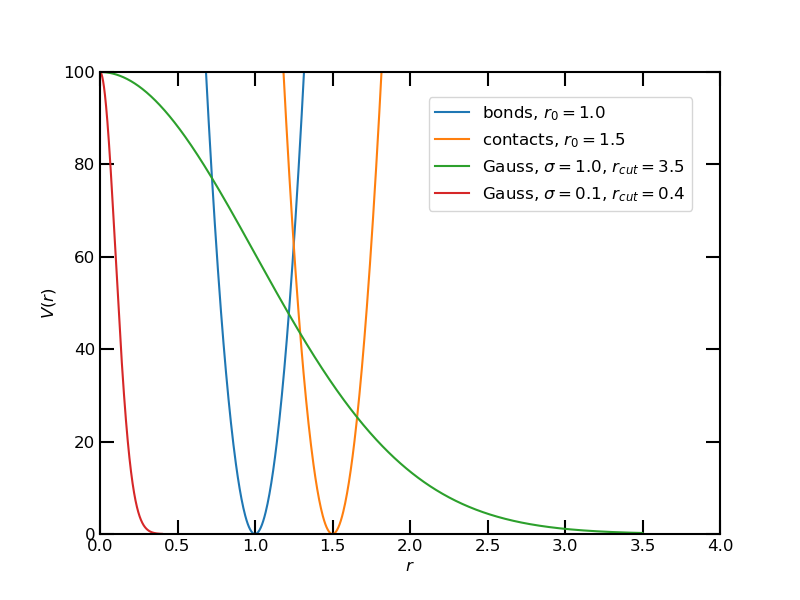
\includegraphics[width=\figwidth]{potentials.png}
  \caption{Potentials used in the simulation. Bonds and contacts are harmonic potentials of the form \(V(r) = 1000 (r - r_0)^2\), with bonds having an \(r_0\) of 1.0 and contacts having an \(r_0\) of 1.5. Gauss potentials are of the form \(V(r) = 100 \exp\left[- \frac{2} \left( \frac{r}{\sigma} \right)^2 \right]\) for \(r\) smaller than \(r_\text{cut}\) and \(0\) for \(r\) greater than the cutoff value \(r_\text{cut}\).}
  \label{fig:potentials}
\end{figure}

The system is initialised by distributing all the beads randomly throughout the simulation box (uniform distribution, using \verb|numpy.uniform.random|\cite{harris_array_2020}). The bonds are set and the simulation is repeatedly cycled through the following steps:

\begin{itemize}[label=\(\bullet\)]
  \item 80,000 time steps with no excluded volume potential
  \item 50,000 time steps with reduced volume potential
  \item 50,000 time steps with full excluded volume potential
\end{itemize}

Bonds and contacts are active at all of those steps. After each cycle the current state is saved to a gsd trajectory file. These saved states will be referred to in the following as \textbf{frames}. Frames whose trajectories are similar are said to have the same \textbf{configuration}. These steps were repeated in each simulation for a total of 105 cycles. The first few cycles have to be discarded as the system takes some time to find its ground state, although certain problems can arise here that will be discussed later in \ref{sec:problems_with_the_simulation}.

% section model_and_simulation_protocol (end)

\section{Simulation results} % (fold)
\label{sec:simulation_results}

Each simulation yields 105 sequential frames, i.e. the simulation state is not reset after each simulation cycle, but instead the final state of the last cycle is the initial state of the next cycle. This has the advantage of giving the system time to tune in, but also the disadvantage of the possibility that certain end configurations will never be reached in a particular simulation run after it has tuned in to a different locally minimal configuration. The potential energies of each frame for the simulation run of cell 2 can be seen in Figure~\ref{fig:potential_energy_cell2}. The first two frames show a potential energy significantly larger than the later ones, then the system quickly converges to a potential energy of about \(\num{7950000}\) and shows only small deviations of less than \(1 \%\) of the mean. Thus both the length of the settling period and the potential energy of the ground configuration match (Wettermann et al.\cite{wettermann_minimal_2020}) extremely well. To minimise the effect of the settling period the first 5 frames of each simulation run will generally be excluded in all subsequent analyses where the data is combined over all frames such as averages or standard deviations.

Furthermore, Figure~\ref{fig:distance_pdf_cell2} shows the distance distribution of the bonds and predetermined contacts combined across all frames of the simulation of cell 2. The results are again very similar to (Wettermann et al.\cite{wettermann_minimal_2020}), with both peaks and means shifted slightly to the right of the respective preferred bond length of \(1.0\) and \(1.5\). The \(99.73\)th quartile is at \(1.71\) for bonds and \(2.42\) for contacts, showing that a substantial portion of the bonds and predetermined contacts are enforced reasonably well.

\begin{figure}[ht]
\centering
  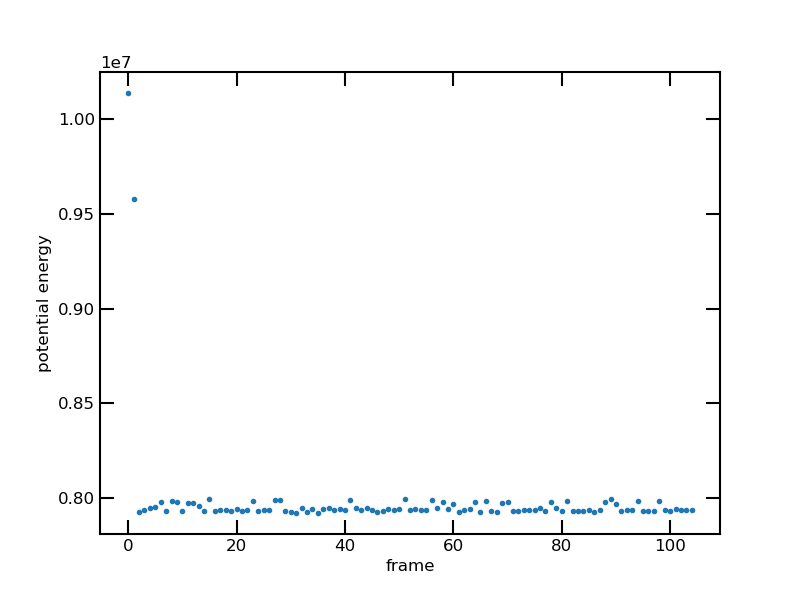
\includegraphics[width=12cm]{potential_energy_cell2.png}
  \caption{Potential energy of each frame in the simulation of cell 2.}
  \label{fig:potential_energy_cell2}
\end{figure}

\begin{figure}[ht]
\centering
  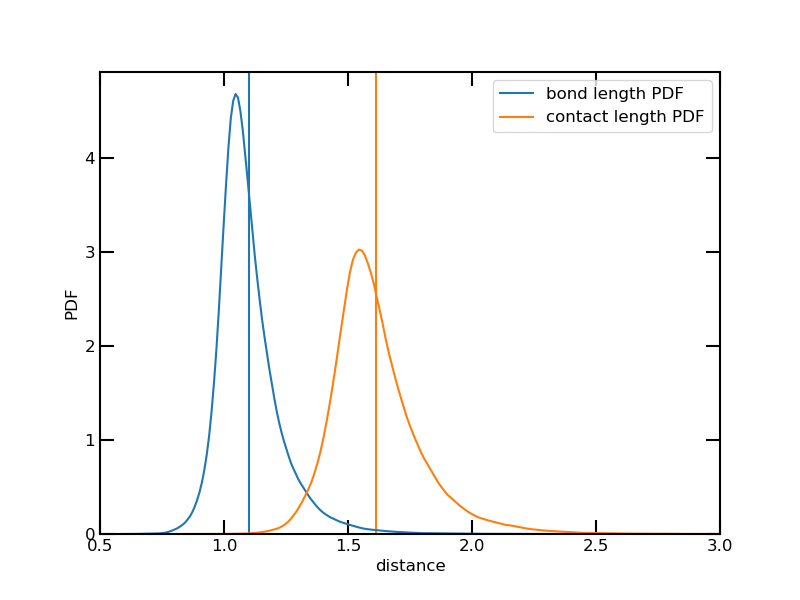
\includegraphics[width=12cm]{distance_pdf_cell2.png}
  \caption{Distance distributions for bonds and predetermined contacts over all frames in the simulation of cell 2 with the means marked by a vertical line. The mean of the bond distances is at \(\num{1.10}\) and the mean of the contact distances is at \(\num{1.61}\).}
  \label{fig:distance_pdf_cell2}
\end{figure}

For the other cells the situation is generally similar, except for cell 1 and cell 5, which will be discussed more in-depth in \ref{sec:problems_with_the_simulation}. The coefficients of variation, i.e. the standard deviations divided by the means, of potential energies are between \(0.3\%\) and \(1.8\%\), showing the minimum energy configuration to be quite stable in these cells. Also neither bonds nor contacts are overly overstretched in any cells, including cell 1 and cell 5. A complete overview of potential energy coefficients of variation and means and \(99.73\)th percentiles for bonds and predefined contacts can be found in Table~\ref{tab:simulation_pe_dists}.

Renderings of all simulated cells can be seen in Appendix~\ref{cha:renderings_of_simuated_cells}. A few things can be notes from these images visually. First, most simulated genomes have a quite regular, spherical shape, but in particular cell 3, cell 8, and the higher energy configuration of cell 5 (which will be discussed in more detail in \ref{sec:problems_with_the_simulation}) show clear differences from this. Cell 3 and cell 8 have a more elongated, bean-like shape, as can be seen in Figure~\ref{img:cell3_frame104_scene1} for cell 3 and in Figure~\ref{img:cell8_frame104_scene2} for cell 8. The higher energy configuration of cell 5 on the other hand has a more obloid, donut-like shape. Also notable is the fact that cell 6 and cell 7 are hollow as can be seen for example in Figure~\ref{img:cell6_frame104_scene1} for cell 6 and Figure~\ref{img:cell7_frame104_scene1} for cell 7. More renderings of all simulated cells can be seen in Appendix \ref{cha:renderings_of_simuated_cells}.

% section simulation_results (end)

\section{Problems with the simulation} % (fold)
\label{sec:problems_with_the_simulation}

While the simulations of most cells quickly reached a stable ground state configuration, the simulations of cell 1 and of cell 5 showed significant deviation from the expected results, warranting further investigation.

\subsection{Cell 1} % (fold)
\label{sub:cell_1}

In cell 1, a ground state is reached very quickly, but this ground state is very unstable, as indicated by the comparably high coefficient of variation of the potential energy of 8.51\% in Table~\ref{tab:simulation_pe_dists} and seen in Figure~\ref{fig:potential_energy_cell1}. The RMSDs of all frames with respect to the last frame as seen in Figure~\ref{fig:rmsd_cell1} shows that some of these frames have rather similar configurations while others are very different. One hypothesis would be that some frames represent a ground state configuration while others are higher energy states. This can be tested by selecting for all frames with low energy, defined by being below some cutoff energy, and checking how the RMSDs for those low-energy frames behaves. A cutoff energy of \(\num{1.495e7}\), visually displayed in Figure~\ref{fig:potential_energy_cell1} as the orange line, was chosen as it captures most of the frames that can be identified visually as being low energy, while excluding all that deviate strongly from this energy baseline. This selects a total of 52 frames, which have been marked in Figure~\ref{fig:rmsd_cell1} by red dot. As can be seen very clearly, these low energy frames do in fact have a low RMSD of \(\num{1.00(1)}\) with respect to the last frame. This confirms that while it is very unstable, this simulation of cell 1 does in fact have a ground state configuration, and it can be filtered for by selecting for those frames with a low energy. To check if this ground state instability is an intrinsic property of the Hi-C contact data for cell 1 or merely a random artefact of this particular simulation run, cell 1 was simulated two more times. The potential energies for those repeated simulations can be seen in Figure~\ref{fig:potential_energy_cell1_1} and Figure~\ref{fig:potential_energy_cell1_2} in the appendix and clearly show the same pattern of instability, leading to the conclusion that this instability is in fact a consequence of the predetermined contacts for cell 1.

\begin{figure}[ht]
\centering
  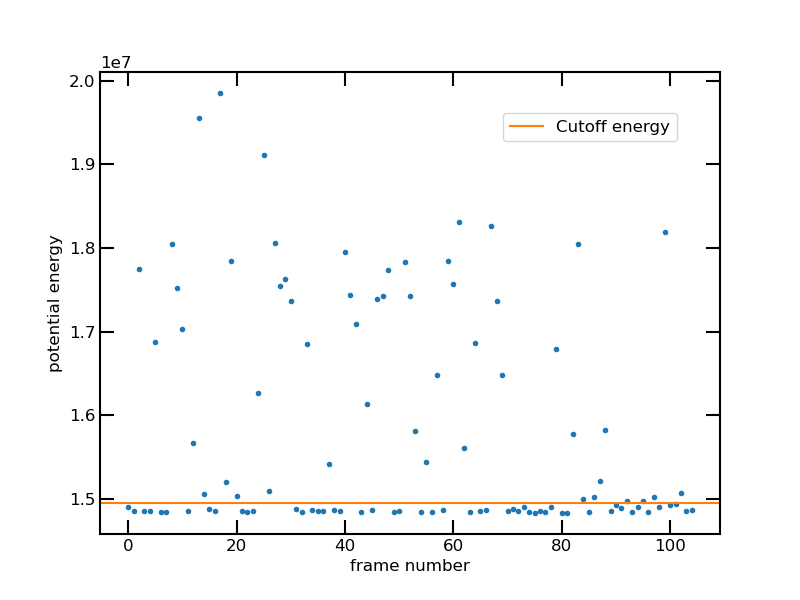
\includegraphics[width=10.5cm]{potential_energy_cell1.png}
  \caption{Potential energies of all frames in the simulation of cell 1. Cutoff energy is set at \(\num{1.495e7}\), with all frames lower than this threshold being defined as \enquote{low-energy frames}.}
  \label{fig:potential_energy_cell1}
\end{figure}

\begin{figure}[ht]
\centering
  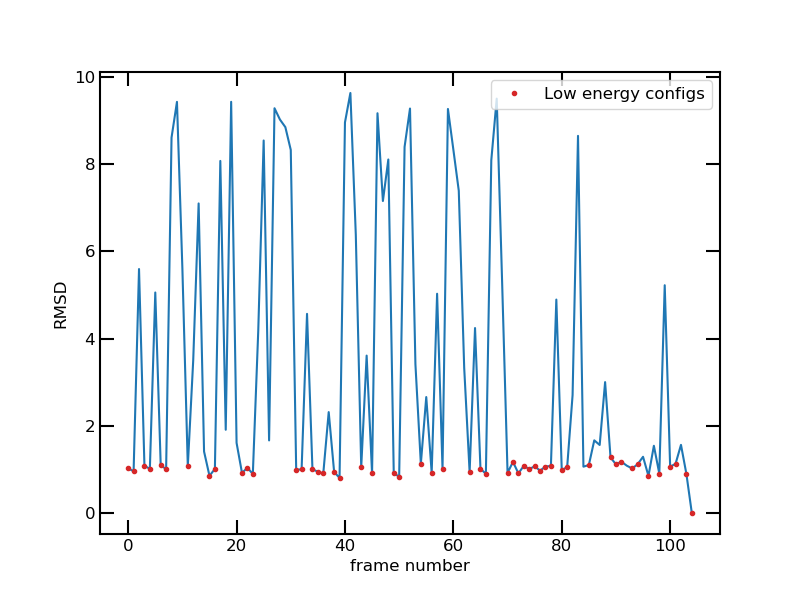
\includegraphics[width=10.5cm]{rmsd_cell1.png}
  \caption{RMSDs of cell 1 with respect to last frame. Low-energy frames, as defined in Figure~\ref{fig:potential_energy_cell1} to be frames with a potential energy lower than \(\num{1.495e7}\), have their RMSD marked by a red dot.}
  \label{fig:rmsd_cell1}
\end{figure}

% subsection cell_1 (end)

\FloatBarrier

\subsection{Cell 5} % (fold)
\label{sub:cell_5}

Figure~\ref{fig:potential_energy_cell5_all} shows the potential energies of all frames in the simulation of cell 5 in blue. As can be seen, after the zeroth frame, which is of higher energy as is typical for the transient phase, the potential energy drops to and stabilises around a value of \(\num{9.805(43)e6}\) for frames 1 through 38. But then for frame 39 and the following ones until the end of the simulation, the energy drops down again to a significantly lower value of \(\num{8.220(8)e6}\). As seen in Figure~\ref{fig:potential_energy_cell5_all}, this is a reduction in both the potential energy itself as well as the deviation in potential energy, from a coefficient of variation of \(0.5 \%\) down to \(0.1 \%\), signifying that the second configuration is both energetically more favourable as well as very stable. The fact that the first configuration was held for 38 frames though means that the existance of semi-stable configurations apart from the ground state configuration is possible. To examine this effect further, cell 5 was simulated 2 more times. The resulting potential energies, together with the potential energies of the first simulation, can be seen in Figure~\ref{fig:potential_energy_cell5_all}. Clearly the second and third simulation run show the same pattern that most other cells exhibit: the first one or two frames have a higher potential energy, and then it drops into a stable ground state configuration where it remains for the rest of the simulation. The very similar potential energies of the ground state configurations in all three simulations suggests that these ground state configurations are in fact the same across all simulations. An analysis of the RMSDs of each frame in all three simulations from the last frame of the first simulation can be seen in Figure~\ref{fig:rmsd_cell5_all} and clearly confirms that the ground states of all three simulations are in fact the same one. This means that while the simulation of cell 5 does have a single stable ground state configuration, it also has a semi-stable configuration that arises in some, but not all simulation runs.

% \begin{figure}[ht]
% \centering
%   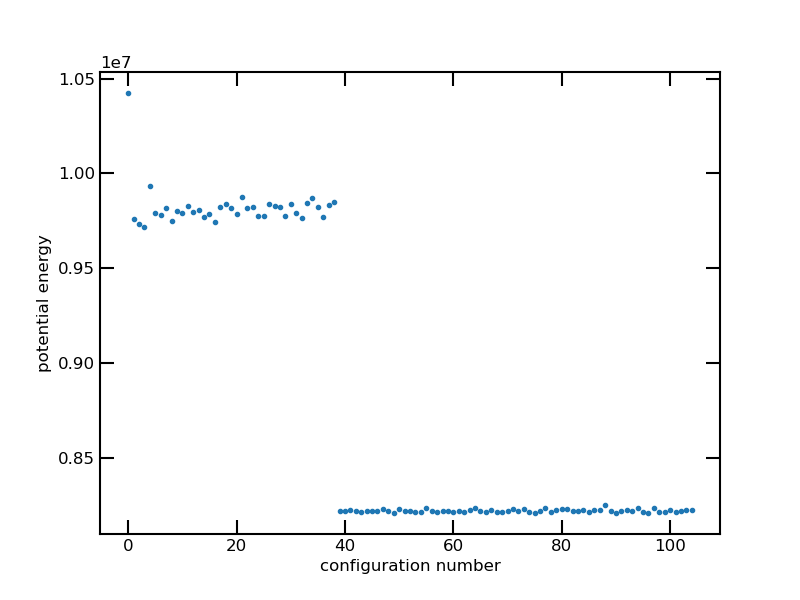
\includegraphics[width=\figwidth]{potential_energy_cell5.png}
%   \caption{Potential energies of all frames in the (first) simulation of cell 5.}
%   \label{fig:potential_energy_cell5}
% \end{figure}

\begin{figure}[ht]
\centering
  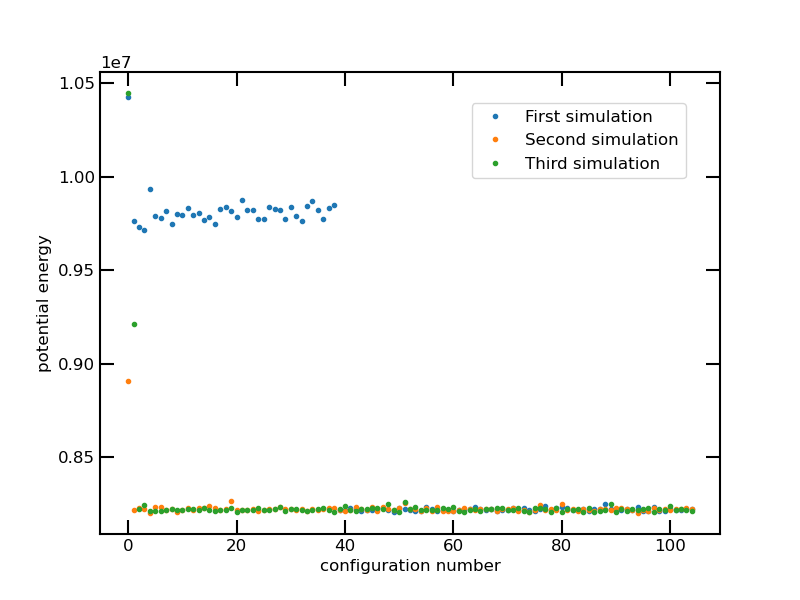
\includegraphics[width=\figwidth]{potential_energy_cell5_all.png}
  \caption{Potential energies of all frames in all three simulations of cell 5.}
  \label{fig:potential_energy_cell5_all}
\end{figure}

\begin{figure}[ht]
\centering
  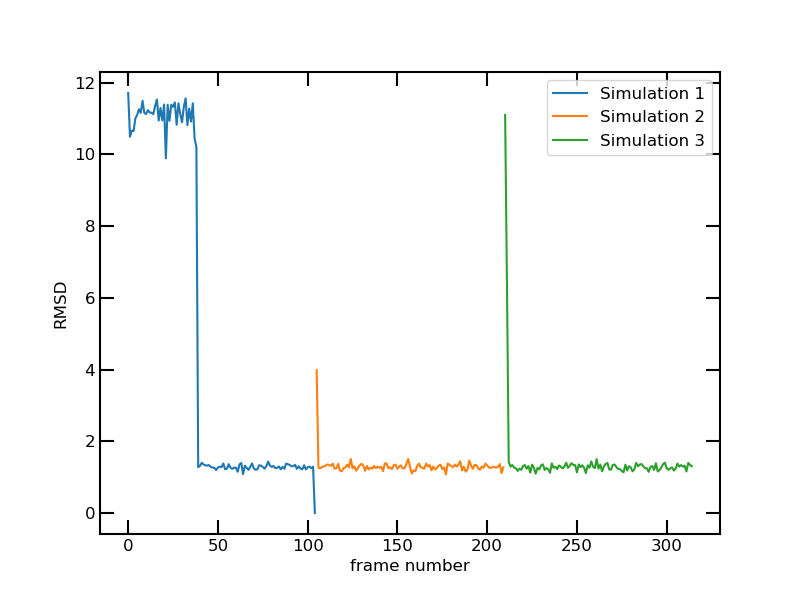
\includegraphics[width=\figwidth]{rmsd_cell5_all.png}
  \caption{RMSD of all three simulations of cell 5 with respect to the last frame of the first simulation.}
  \label{fig:rmsd_cell5_all}
\end{figure}

% subsection cell_5 (end)

% section problems_with_the_simulation (end)


% chapter simulation (end)


%_______________________________________________________________________________


%!TEX root = ../thesis

\chapter{Comparison of Cells} % (fold)
\label{cha:comparison_of_cells}

\section{Definition of SCC} % (fold)
\label{sec:definition_of_scc}

HiCRep is a mathematical tool introduced in (Yang et al.\cite{yang_hicrep_2017}) for the explicit purpose of comparing Hi-C data sets. It takes as input the contact matrices of two Hi-C data sets (or, more generally, contact matrices of any kind) and outputs a correlation coefficient, that is a number between \(-1\) and \(1\), with larger numbers signifying a stronger similarity between the data sets and vice versa. This is done in a two-step process: first both contact matrices are smoothed to counteract binning-associated problems and then a stratum-adjusted correlation coefficient (SCC) is calculated between these smoothed contact matrices. The exact procedure will be explained in the following section.

\subsection{Smoothing} % (fold)
\label{subsec:smoothing}

Both contact maps are first smoothed using a square uniform filter of width \(2h+1\) for a chosen smoothing parameter \(h \geq 0\). This helps compensating a lack of coverage, that is the fact that not all physical contacts are contained in the contact matrices, a common problem for Hi-C data. Mathematically this filter can be defined as

\[
  X_{ij} = \frac{ \sum_{k=i-h}^{i+h} \sum_{l=j-h}^{j+h} C_{kl} }{ 2h+1 }
\]

where \(C\) is the \(n \times n\) raw contact matrix and \(X\) is the \(n \times n\) smoothed contact matrix. \(C_{ij}\) is defined to be 0 for either \(i\) or \(j\) not in \(\set{1, \dots, n}\).

The uniform filter might seem like an unusual choice compared to other more sophisticated filters, but it has the great advantage of having the representation \( X = L \cdot C \cdot R \), where \(X\) is the smoothed matrix, \(C\) is the raw contact matrix, and \(L\) and \(R\) are upper and lower triangular matrices respectively. This is useful for computational purposes, especially when using sparse representations of \(C\) and \(X\), which is recommended since contact matrices generally can be quite large, 25,714\(\times\)25,714 in this case, but are mostly empty.

\(h\) is a parameter for the SCC algorithm and thus has to be chosen appropriately. The HiCRep package includes a function called \verb|htrain| (\verb|h_train| in the HiCRep.py Python package) that tries to estimate an appropriate h-value heuristically. For a resolution of \(\SI{100}{kbp}\) an example value of \( h = 3 \) is given in the original HiCRep paper, which should be kept in mind as a refence when trying to choose an h-value later.

% subsection smoothing (end)

\subsection{SCC} % (fold)
\label{subsec:scc}

The stratum-adjusted correlation coefficient aims to be a measure of correlation between two random variables \(X\) and \(Y\) that are stratified by a third variable into \(K\) strata \(X_1, \dots, X_K\) and \(Y_1, \dots, Y_K\) respectively. In each stratum there are the stratified random variables \((X_k, Y_k)\) with \(N_k\) observations \( (x_{k,1}, y_{k,1}), \dots, (x_{k,N_k}, y_{k,N_k}) \) each. The pearson correlation coefficient between \(X\) and \(Y\) for the k-th stratum is given by

\[
  \rho_k = \frac{ \mathrm{Cov}(X_k,Y_k) }{ \sqrt{ \mathrm{Var}(X_k) \mathrm{Var}(Y_k)} } = \frac{ \sum_{i=1}^{N_k} (x_{k,i} - \overbar{x}_k) (y_{k,i} - \overbar{y}_k) }{ \sqrt{ \sum_{i=1}^{N_k} x_{k,i} - \overbar{x}_k } \sqrt{ \sum_{i=1}^{N_k} y_{k,i} - \overbar{y}_k } }
\]

The SCC is the weighted average of the pearson correlation coefficients of the different strata:

\[
  \rho_s = \sum_{k=1}^{K} w_k \rho_k
\]

where the weights \(w_k\) are given by

\[
  w_k = \sqrt{ \mathrm{Var}\left( \frac{ \mathrm{Rank}(X_k) }{ N_k } \right) \mathrm{Var}\left( \frac{ \mathrm{Rank}(Y_k) }{ N_k } \right) }
\]

with \( \mathrm{Rank}(X_k) \) and \( \mathrm{Rank}(Y_k) \) being the ranked variables\footnote{\url{https://en.wikipedia.org/wiki/Ranking\#Ranking_in_statistics}} of \(X_k\) and \(Y_k\) respectively. For a thorough derivation of the SCC see the original \mbox{HiCRep} paper\cite{yang_hicrep_2017}, Section \enquote{Derivation of stratum-adjusted correlation coefficient (SCC)}.

% section definition_of_scc (end)

\section{SCC between cells} % (fold)
\label{sec:scc_between_cells}

In Figure~\ref{fig:hic_vs_sim_scc} the SCC between the original Hi-C contact matrices and the contact matrices of the simulation can be seen for each cell. Two beads in the simulation were defined to be in contact if their distance is less than \(3.0\) and contacts were counted across all frames. For all cells the SCC is between 0.68 and 0.80. This is sensible since on one hand, the SCC is expected to be high as the simulated data is based on the Hi-C data, on the other hand it is not surprising that the scores are not perfect since the Hi-C data doesn’t cover all contacts in the real genome whereas the simulation data includes all contacts in the simulated genome. Particularly interesting is that the SCCs for cell 1 and cell 5 are very much in line with those of the other cells, regardless of the problems that have arisen during the simulation and were discussed in \ref{sub:cell_1} and \ref{sub:cell_5} respectively. This could indicate either that regardless of their problems cell 1 and cell 5 replicated the contacts or their Hi-C data as well or that all simulations replicated the Hi-C data badly so that there is no recognisable difference. This question can unfortunately not be answered here.

The pairwise SCC between the original Hi-C data of all cells can be seen in Table~\ref{tab:scc_hic}. It is immediately very clear that all SCC values (except for those of a cell with itself) are very low, especially compared to the values of \(0.7\) to \(1.0\) obtained in the original HiCRep paper for hESC (human embryonic stem cells) and IMR90 (human lung fibroblast cells) cell lines (Figure~3A in \cite{yang_hicrep_2017}). This might very likely be related to the fact that each of the Hi-C data sets that have been used for this analysis captured only an estimated \(5\%\) of all physical contacts in the actual cell, as detailed in Table~\ref{tab:contact_capture}, but regardless of the reasons, it sets the expectations for similarity between the simulated cells quite low. The SCC for the contact matrices of the simulated genomes can be seen in Table~\ref{tab:scc_sim} and, as was expected, are similarly low to those of the initial Hi-C contact matrices. This strongly suggests that the structure of the simulated genomes have very little relation with each other. This assumption is also backed by the rendered images in \ref{cha:renderings_of_simuated_cells} that show the simulated genomes differ quite strongly in shape, e.g. with some being spherical and others being bean-shaped or obloid, or some of them having some rather big holes inside them making them basically hollow. In summary, the low SCCs are a first strong indicator that the global structure of the different simulated genomes are significantly different.

\begin{table}[ht]
\centering
  \sisetup{ table-alignment-mode=none }
  \caption{SCC calculated pairwise between the contact matrices of the original Hi-C data. Contacts are binned to a size of \(\SI{100000}{bp}\) per bin. Multiple contacts between the same bins are only counted once. The smoothing parameter \(h\) is set to \(7\). The SCC between a cell and itself is always \(1.0\) and thus omitted.}
  \label{tab:scc_hic}
  \begin{tabular}{S | S S S S S S S S}
   & {Cell 1} & {Cell 2} & {Cell 3} & {Cell 4} & {Cell 5} & {Cell 6} & {Cell 7} & {Cell 8} \\
  \midrule
    {Cell 1} &  {-}  & 0.132 & 0.093 & 0.116 & 0.128 & 0.105 & 0.136 & 0.092 \\
    {Cell 2} & 0.132 &  {-}  & 0.098 & 0.104 & 0.147 & 0.116 & 0.150 & 0.138 \\
    {Cell 3} & 0.093 & 0.098 &  {-}  & 0.062 & 0.104 & 0.093 & 0.101 & 0.092 \\
    {Cell 4} & 0.116 & 0.104 & 0.062 &  {-}  & 0.108 & 0.101 & 0.123 & 0.077 \\
    {Cell 5} & 0.128 & 0.147 & 0.104 & 0.108 &  {-}  & 0.121 & 0.148 & 0.123 \\
    {Cell 6} & 0.105 & 0.116 & 0.093 & 0.101 & 0.121 &  {-}  & 0.145 & 0.097 \\
    {Cell 7} & 0.136 & 0.150 & 0.101 & 0.123 & 0.148 & 0.145 &  {-}  & 0.116 \\
    {Cell 8} & 0.092 & 0.138 & 0.092 & 0.077 & 0.123 & 0.097 & 0.116 &  {-}  \\
  \end{tabular}
\end{table}

\begin{table}[ht]
\centering
  \sisetup{ table-alignment-mode=none }
  \caption{SCC calculated pairwise between the contact matrices of the simulated structures. Two beads are defined to be in contact if their distance from the centre is less than 3. The smoothing parameter \(h\) is set to \(7\). The SCC between a cell and itself is always \(1.0\) and thus omitted.}
  \label{tab:scc_sim}
  \begin{tabular}{S | S S S S S S S S}
   & {Cell 1} & {Cell 2} & {Cell 3} & {Cell 4} & {Cell 5} & {Cell 6} & {Cell 7} & {Cell 8} \\
  \midrule
    {Cell 1} &  {-}  & 0.171 & 0.149 & 0.114 & 0.173 & 0.141 & 0.178 & 0.104 \\
    {Cell 2} & 0.171 &  {-}  & 0.164 & 0.141 & 0.183 & 0.184 & 0.215 & 0.184 \\
    {Cell 3} & 0.149 & 0.164 &  {-}  & 0.109 & 0.161 & 0.124 & 0.145 & 0.122 \\
    {Cell 4} & 0.114 & 0.141 & 0.109 &  {-}  & 0.135 & 0.105 & 0.140 & 0.098 \\
    {Cell 5} & 0.173 & 0.183 & 0.161 & 0.135 &  {-}  & 0.148 & 0.194 & 0.143 \\
    {Cell 6} & 0.141 & 0.184 & 0.124 & 0.105 & 0.148 &  {-}  & 0.191 & 0.116 \\
    {Cell 7} & 0.178 & 0.215 & 0.145 & 0.140 & 0.194 & 0.191 &  {-}  & 0.157 \\
    {Cell 8} & 0.104 & 0.184 & 0.122 & 0.098 & 0.143 & 0.116 & 0.157 &  {-}  \\
  \end{tabular}
\end{table}

\FloatBarrier

% section scc_between_cells (end)

\section{RMSD between cells} % (fold)
\label{sec:rmsd_between_cells}

Another way to gauge the similarity of the configurations between the simulated genomes is to calculate RMSDs between the configurations of the cells. There are generally two straightforward approaches that can be taken when calculating RMSDs between the different cells: first,  a reference frame can be chosen for each cell and the RMSDs between these reference frames can be calculated. While this approach is very direct, it does strongly depend on the choice of a good reference frame and is generally much more susceptible to statistical variation between the different frames of a simulation run. The other approach would be to calculate an average trajectory from all (or, as will be discussed, only certain selected) frames in a cell and then calculate the RMSDs between those average trajectories. While this counteracts the statistical problems of using a reference frame, it has a challenge of its own: it only makes sense to take the average of frames that represent the same configuration, i.e. that are already similar to each other. In particular, this not the case for example for the simulation of cell 5, which contains, as discussed in \ref{sub:cell_5}, two configurations, one ground state configuration and one of higher energy, or similarly the simulation of cell 1 which contains besides the ground state frames a number of higher energy frames. To calculate average trajectories, it needs to be ensured that the frames that are averaged over are sufficiently similar and all represent the ground configuration while carefully filtering out the rest.

 For cell 1 the same energy-filtering approach was chosen as in \ref{sub:cell_1} to select only those frames with ground state energy. For cell 5 only frames 39 and onward were included as those represent the ground state frames of the simulation. For the other cells simply the first 5 frames were excluded to avoid the tune-in period as discussed in \ref{sec:simulation_results}. The resulting RMSDs of each frame to both a reference frame, here the last frame of each simulation, and the average trajectory is shown in Figure~\ref{fig:rmsd_last_vs_avg}. There are two major things than can be learned from Figure~\ref{fig:rmsd_last_vs_avg}: first, the RMSD from average is quite consistently smaller than the RMSD from last, implying the averaged trajectories fulfil their purpose as representations of the ground state configuration well. Second, for all cells except cell 1 and cell 5 the mean of the RMSDs from the average trajectory seen in Table~\ref{tab:mean_std_rmsd_from_avg} is between \(0.9\) and \(1.9\), with standard deviations mostly between \(0.08\) and \(0.23\), with the only exception being cell 4 with a slightly higher standard deviation of  \(0.66\). For cell 1 and cell 5 the raw means and standard deviations are significantly larger due to the presence of the non ground configuration frames, but after applying the filtering from above the means drop to \(\num{0.68(10)}\) and \(\num{0.88(7)}\) respectively, although this is expected as precisely those frames get filtered out that showed strong deviation from the ground state configuration the averaged trajectory is representing. The unexpected outlier here is cell 4 with a mean RMSDs to average of \(\num{1.55(66)}\) and several pronounced spikes seen in Figure~\ref{fig:rmsd_last_vs_avg}. Looking at the potential energies of the frames with spikes shows that those frames have somewhat elevated potential energy compared to the other frames. Filtering out the nine most promimently spiked frames improves the mean RMSD to average of cell 4 to \(\num{1.36(19)}\), making it fall more in line with the other cells. This improvement is, especially for the standard deviation, significant enough to use this filtering from here on.

\begin{table}[ht]
\centering
  \caption{Mean and standard deviation of the RMSDs of each frame to the average trajectory for each cell simulation.}
  \label{tab:mean_std_rmsd_from_avg}
  \begin{tabular}{l S S S S S S S S}
  \toprule
    Cell & {1} & {2} & {3} & {4} & {5} & {6} & {7} & {8} \\
  \midrule
    RMSD Mean & 3.54 & 0.90 & 0.95 & 1.55 & 5.07 & 1.37 & 1.88 & 1.78 \\
    RMSD Std & 2.46 & 0.16 & 0.23 & 0.66 & 2.58 & 0.21 & 0.12 & 0.08 \\
  \bottomrule
  \end{tabular}
\vspace{0.4cm}
\end{table}

 Using the filterings described above to generate the average trajectory for each cell, the RMSDs between each of them can be seen in Table~\ref{tab:rmsd_avg_between_cells}. Except for the self-RMSDs they are all between \(18.4\) and \(25.0\), implying the average whole genome trajectories for each cell simulation are significantly different, affirming the same conclusion made in \ref{sec:scc_between_cells} using the genome level SCC.

\begin{table}[ht]
\centering
  \caption{RMSDs between average trajectories of each cell. Each average trajectory is generated from the ground state frames of the simulations. The RMSD between a cell and itself is always \(0\) and thus omitted.}
  \label{tab:rmsd_avg_between_cells}
  \begin{tabular}{S | S S S S S S S S}
  % \toprule
     & {Cell 1} & {Cell 2} & {Cell 3} & {Cell 4} & {Cell 5} & {Cell 6} & {Cell 7} & {Cell 8} \\
  \midrule
    {Cell 1} &  {-} & 19.4 & 19.8 & 18.4 & 19.2 & 19.6 & 23.7 & 24.3 \\
    {Cell 2} & 19.4 &  {-} & 18.9 & 18.4 & 19.6 & 20.1 & 24.5 & 24.1 \\
    {Cell 3} & 19.7 & 18.9 &  {-} & 18.4 & 19.5 & 19.9 & 22.1 & 23.9 \\
    {Cell 4} & 18.4 & 18.4 & 18.4 &  {-} & 19.1 & 19.3 & 24.5 & 24.5 \\
    {Cell 5} & 19.2 & 19.6 & 19.5 & 19.1 &  {-} & 19.6 & 25.0 & 23.4 \\
    {Cell 6} & 19.7 & 20.1 & 19.9 & 19.3 & 19.6 &  {-} & 23.9 & 22.6 \\
    {Cell 7} & 23.7 & 24.5 & 22.1 & 24.5 & 25.0 & 23.9 &  {-} & 24.4 \\
    {Cell 8} & 24.3 & 24.1 & 23.9 & 24.5 & 23.4 & 22.6 & 24.4 &  {-} \\
  % \bottomrule
  \end{tabular}
\end{table}

% section rmsd_between_cells (end)

% chapter comparison_of_cells (end)


%_______________________________________________________________________________


%!TEX root = ../thesis

\chapter{Individual Chromosomes} % (fold)
\label{cha:individual_chromosomes}

\section{RMSDs between individual chromosomes} % (fold)
\label{sec:rmsds_between_individual_chromosomes}

The comparison of the simulated structure between cells can be made on the chromosome level instead of the entire genome level. The results can be seen in Table~\ref{tab:mean_chrom_cross_rmsd}. While the mean RMSDs are significantly smaller than for the entire-genome case, they are still high enough to suggest no real similarity between the chromosomes across all cells, and the decrease can be explained simply by the smaller number of constraints when aligning the two trajectories. Considering even the minimum RMSD of each chromosome is never smaller than \(4.7\), it can be concluded that very likely there is no significant similarity between each chromosome across the different cells.

\begin{table}[ht]
\centering
  \caption{Mean and minimum of RMSDs of a particular chromosome pairwise between the averaged trajectories of all cells, excluding self-comparisons.}
  \label{tab:mean_chrom_cross_rmsd}
  \begin{tabular}{l @{\phantom{abc}} S S S S S S S S S S}
  \toprule
    Chrom & {1} & {2} & {3} & {4} & {5} & {6} & {7} & {8} & {9} & {10} \\
    Mean RMSD & 9.6 & 8.1 & 8.4 & 8.3 & 8.1 & 7.5 & 8.3 & 8.0 & 8.1 & 7.9 \\
    Min RMSD  & 6.8 & 6.5 & 5.6 & 5.3 & 6.1 & 5.9 & 5.9 & 6.0 & 6.3 & 4.9 \\
  \midrule
    Chrom & {11} & {12} & {13} & {14} & {15} & {16} & {17} & {18} & {19} & {X} \\
    Mean RMSD & 7.8 & 8.2 & 8.6 & 8.4 & 7.1 & 7.4 & 7.3 & 6.9 & 7.0 & 8.7 \\
    Min RMSD  & 6.6 & 5.6 & 5.6 & 5.6 & 5.4 & 5.3 & 5.5 & 5.0 & 4.7 & 6.7 \\
  \bottomrule
  \end{tabular}
\end{table}

% section rmsds_between_individual_chromosomes (end)

\section{Simulation of individual chromosomes} % (fold)
\label{sec:simulation_of_individual_chromosomes}

Instead of simulating the entire genome, only individual chromosomes can be simulated in isolation. This can show how much of the structure of each chromosome is dependent on intrinsic interactions in the chromosome itself opposed to extrensic interactions with other chromosomes. Simulations were carried out for chromosome 1 and chromosome 19, as those are the largest and smallest chromosome respectively.

\subsection{Chromosome 1} % (fold)
\label{ssec:chromosome_1}

In Figure~\ref{fig:potential_energy_cell3_chrom1} the potential energy for the simulation of chromosome 1 of cell 3 is displayed. Compared to the potential energy of cell 2 in Figure~\ref{fig:potential_energy_cell2} the potential energies for the invdividual chromosome look a lot more spread out and unstable, but the coefficient of variation of the potential energy of \(1.24 \%\) is actually comparably low in reference to the coefficients of variation of the cell simulations as seen in Table~\ref{tab:simulation_pe_dists}. 

\begin{figure}[ht]
\centering
	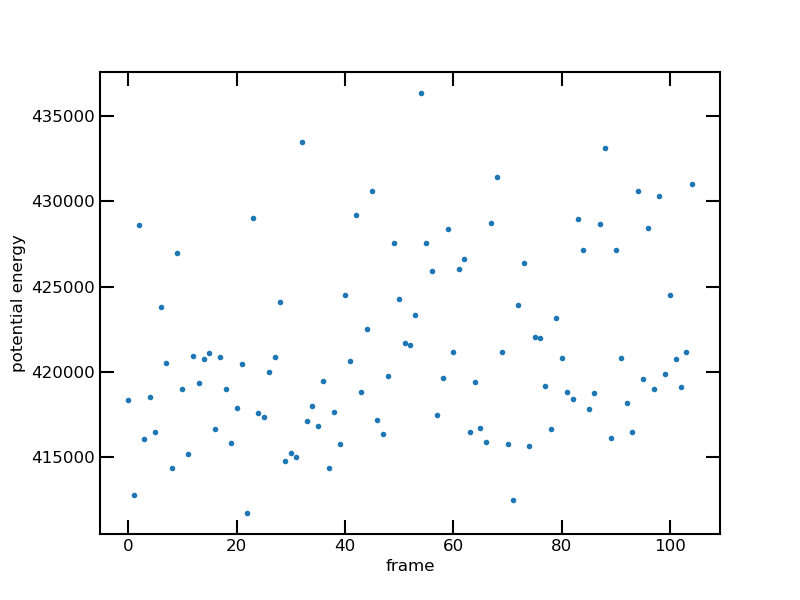
\includegraphics[width=\figwidth]{potential_energy_cell3_chrom1.png}
	\caption{Potential energy of all frames for simulation of chromosome 1 of cell 3 indiviually.}
	\label{fig:potential_energy_cell3_chrom1}
\end{figure}

Looking at the RMSDs of the chromsome simulation though, seen in Figure~\ref{fig:potential_energy_cell3_chrom1}, the mean RMSD from frame 22, which is the lowest potential energy frame, is quite high at \(\num{4.6(10)}\). Even worse, even though frame 1 and frame 71 have a similarly low energy compared to frame 22, their respective RMSDs from frame 22 are still larger than \(3.0\), implying that neither of these frames represents a true ground state. The mean RMSDs from the respective lowest energy frame for the simulations of chromosome 1 for all cells in Table~\ref{tab:chrom1_mean_rmsds} show that this is the case for all cells. Unsurprisingly, when comparing these individually simulated chromosomes with their respective counterparts in the simulations of the entire genome, by calculating the RMSD from the chromosome in the average trajectory, the results are similarly bad. This implies that the structure of chromosome 1 when simulated individually is quite dissimilar to the structure when simulated in the context of the entire cell.

\begin{figure}[ht]
\centering
	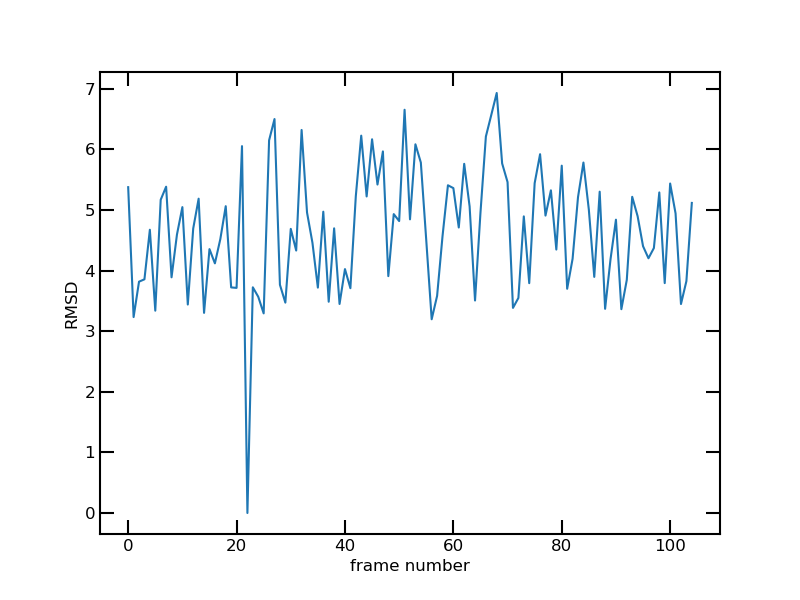
\includegraphics[width=\figwidth]{rmsd_cell3_chrom1.png}
	\caption{RMSD of each frame of the simulation of chromosome 1 of cell 3 with the lowest-energy frame, frame 22.}
	\label{fig:rmsd_cell3_chrom1}
\end{figure}

\begin{table}[ht]
\centering
  \caption{Mean of RMSDs between each frame of chrosomome 1 simulation to lowest energy frame of this simulation and to chromosome 1 in the average trajectory of the entire cell simulation for each cell.}
  \label{tab:chrom1_mean_rmsds}
  \sisetup{ table-alignment-mode=none }
  \begin{tabular}{l @{\phantom{abc}} S S S S S S S S}
  \toprule
    Cell & 1 & 2 & 3 & 4 & 5 & 6 & 7 & 8 \\
  \midrule
    \parbox{4cm}{Mean RMSD to \\ lowest energy frame} & 4.6 & 3.4 & 4.6 & 2.5 & 4.2 & 3.2 & 4.9 & 8.2 \\
    Mean RMSD to avg cell & 4.6 & 3.9 & 5.6 & 3.1 & 4.6 & 6.8 & 5.1 & 7.8 \\
  % \midrule
  %   Internal contacts & 3735 & 2594 & 1231 & 3197 & 2323 & 2860 & 1599 & 1310 \\
  %   External contacts & 1562 & 660 & 854 & 384 & 849 & 294 & 300 & 349 \\
  %   \parbox{4cm}{\centering Proportion of \\ internal contacts} & 71\% & 80\% & 59\% & 89\% & 73\% & 91\% & 84\% & 79\% \\
  \bottomrule
  \end{tabular}
\end{table}

% subsection chromosome_1 (end)

\FloatBarrier

\subsection{Chromosome 19} % (fold)
\label{ssec:chromosome_19}

The same analysis has been repeated for chromosome 19, which is the shortest chromosome with only 584 beads compared to chromosome 1 with 1924 beads. For the RMSDs from the minimum energy frame, displayed in \ref{fig:rmsd_cell3_chrom19}, we see the same pattern as already for chromosome 1, with the RMSD being both very high and unstable. In particular no stable ground state configuration is reached again. The RMSDs to the average trajectory from the entire genome simulation can be seen in Table~\ref{tab:chrom19_mean_rmsds}. While most of the RMSDs are similarly high, for cell 1 and cell 4 the mean RMSD to the average simulated cell drops to \(2.3\) and \(1.5\) respectively, which is indicative of decent resemblance. Nevertheless, generally the difference between the individually simulated chromosomes and the chromosomes in the cell is still quite high, suggesting that the results of cell 1 and cell 4 are merely the exception from the rule and that the stabilising effect of other chromosomes is a non-neglegible factor for determining a chromosome's structure.

\begin{figure}[ht]
\centering
  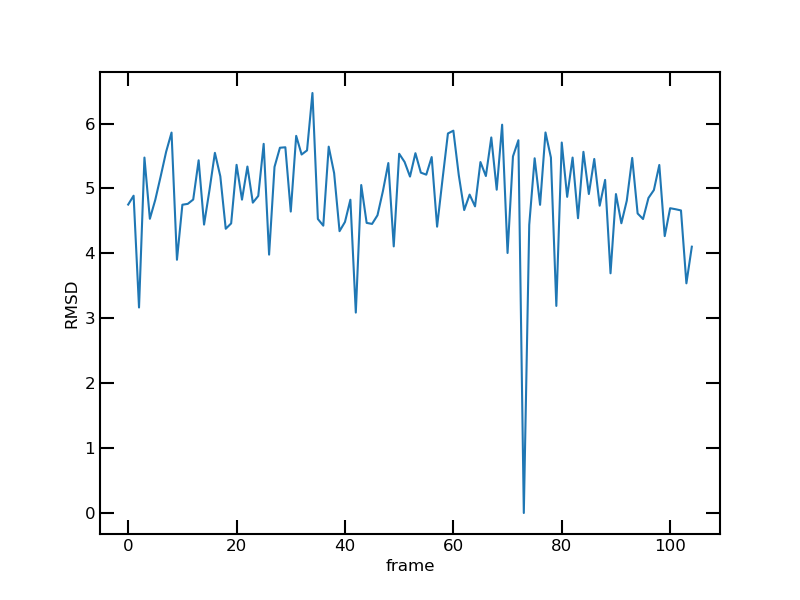
\includegraphics[width=\figwidth]{rmsd_cell3_chrom19.png}
  \caption{RMSD of each frame of the simulation of chromosome 19 of cell 3 with the lowest-energy frame, frame 73.}
  \label{fig:rmsd_cell3_chrom19}
\end{figure}

\begin{table}[ht]
\centering
  \caption{Mean of RMSDs between each frame of chrosomome 19 simulation to lowest energy frame of this simulation and to chromosome 19 in the average trajectory of the entire cell simulation for each cell.}
  \label{tab:chrom19_mean_rmsds}
  \sisetup{ table-alignment-mode=none }
  \begin{tabular}{l @{\phantom{abc}} S S S S S S S S}
  \toprule
    Cell & 1 & 2 & 3 & 4 & 5 & 6 & 7 & 8 \\
  \midrule
    \parbox{4cm}{Mean RMSD to \\ lowest energy frame} & 1.8 & 3.7 & 4.9 & 1.2 & 3.6 & 2.5 & 4.6 & 5.9 \\
    Mean RMSD to avg cell & 2.3 & 4.1 & 6.0 & 1.5 & 4.4 & 3.1 & 4.8 & 6.1 \\
  % \midrule
  %   Internal contacts & 1229 & 717 & 243 & 1037 & 684 & 761 & 460 & 333 \\
  %   External contacts & 605 & 394 & 544 & 214 & 381 & 302 & 142 & 169 \\
  %   \parbox{4cm}{\centering Proportion of \\ internal contacts} & 67\% & 65\% & 31\% & 83\% & 64\% & 72\% & 76\% & 66\% \\
  \bottomrule
  \end{tabular}
\end{table}

% subsection chromosome_19 (end)

% section simulation_of_individual_chromosomes (end)

% One possible explanation for the dissimililarity betwen the chrosomosome structure in the cell and individually could be that the chromosome structure gets stabilised by its contacts with other chromosomes. To examine the strength of this effect the number of Hi-C contacts of the chromosome both with itself and and with other contacts and then calculate the ratio of internal contacts.

% chapter individual_chromosomes (end)


%_______________________________________________________________________________
\chapter{Conclusion} % (fold)
\label{cha:conclusion}

In der Zusammenfassung sollten Sie in knapper Form die Aufgabenstellung 
und die wichtigsten Ergebnisse rekapitulieren. Es ist für die 
Gutachter hilfreich, wenn Sie ausdrücklich beschreiben, worin 
Ihre eigenen Beiträge liegen. Scheuen Sie sich auch nicht davor 
auszusprechen, welche Untersuchungen durch die Zeitbegrenzung der 
Bachelorarbeit nicht möglich waren und nutzen Sie dies als 
überleitung zu einem Ausblick auf mögliche weitergehende 
Arbeiten an der Aufgabenstellung.

% chapter conclusion (end)

\printbibliography

%_______________________________________________________________________________
\appendix

% \chapter{Appendix}
\chapter{Tables and Figures} % (fold)
\label{cha:tables_and_figures}

\medskip

\begin{table}[H]
\centering
  \caption{Number of beads in each chromosome in the simulation. Each bead represents \(\SI{100}{kbp}\)}
  \label{tab:chrom_lengths}
  \begin{tabular}{c c c c c c c c c c c}
   \toprule
    Chrom & 1 & 2 & 3 & 4 & 5 & 6 & 7 & 8 & 9 & 10 \\
    Length & 1924 & 1791 & 1570 & 1534 & 1488 & 1466 & 1424 & 1263 & 1215 & 1275 \\
  \midrule
    Chrom & 11 & 12 & 13 & 14 & 15 & 16 & 17 & 18 & 19 & X \\
    Length & 1189 & 1171 & 1174 & 1218 & 1010 & 952 & 919 & 876 & 584 & 1671 \\
  \bottomrule
  \end{tabular}
\end{table}

\begin{table}[ht]
\centering
  \caption{Some statistics about each simulated cell. The pot(ential) energy \% deviation describes the standard deviation of the potential energy divided by the mean potential energy over all frames except for the first 5. For both bonds and contacts the mean and 99.73th percentile are of the distances between the \emph{predefined} bonds and contacts, i.e. only the ones we set as input before our simulation, not the ones arising in the simulation.}
  \label{tab:simulation_pe_dists}
  \sisetup{ table-alignment-mode=none }
  \begin{tabular}{c @{\phantom{abc}} S @{\phantom{abc}} S @{\phantom{abc}} S @{\phantom{abc}} S @{\phantom{abc}} S}
  \toprule
     & & \multicolumn{2}{c}{bond lengths} & \multicolumn{2}{c}{contact lengths} \\
   \cmidrule(rl){3-4}
   \cmidrule(rl){5-6}
    {Cell} & \parbox{3cm}{\centering pot energy \\ \% deviation} & {mean} & \parbox{3cm}{\centering 99.73th \\ percentile} & {mean} & \parbox{3cm}{\centering 99.73th \\ percentile} \\
  \midrule
    1 & 8.51\% & 1.13 & 1.98 & 1.62 & 2.72 \\
    2 & 0.27\% & 1.10 & 1.71 & 1.61 & 2.42 \\
    3 & 0.67\% & 1.14 & 1.88 & 1.68 & 2.52 \\
    4 & 1.83\% & 1.14 & 2.08 & 1.61 & 2.46 \\
    5 & 8.63\% & 1.11 & 1.81 & 1.62 & 2.55 \\
    6 & 0.94\% & 1.16 & 2.07 & 1.61 & 2.38 \\
    7 & 0.29\% & 1.10 & 1.58 & 1.59 & 2.09 \\
    8 & 0.28\% & 1.08 & 1.56 & 1.60 & 2.25 \\
  \bottomrule
  \end{tabular}
\end{table}

\begin{table}[ht]
\centering
  \caption{caption}
  \label{tab:contact_capture}
  \sisetup{ table-alignment-mode=none }
  \begin{tabular}{S S S S}
  \toprule
    {Cell} & \parbox{3cm}{\centering contacts specified} & \parbox{3cm}{\centering contacts after simulation} & \parbox{3cm}{\centering \% of contacts specified} \\
  \midrule
    1 & 48962 & 932831 & 5.2\% \\
    2 & 32243 & 558981 & 5.8\% \\
    3 & 19112 & 602439 & 3.2\% \\
    4 & 35514 & 685314 & 5.2\% \\
    5 & 31180 & 592569 & 5.3\% \\
    6 & 32862 & 358721 & 4.8\% \\
    7 & 21126 & 358721 & 5.9\% \\
    8 & 17581 & 320656 & 5.5\% \\
  \bottomrule
  \end{tabular}
\end{table}

\begin{figure}[ht]
\centering
  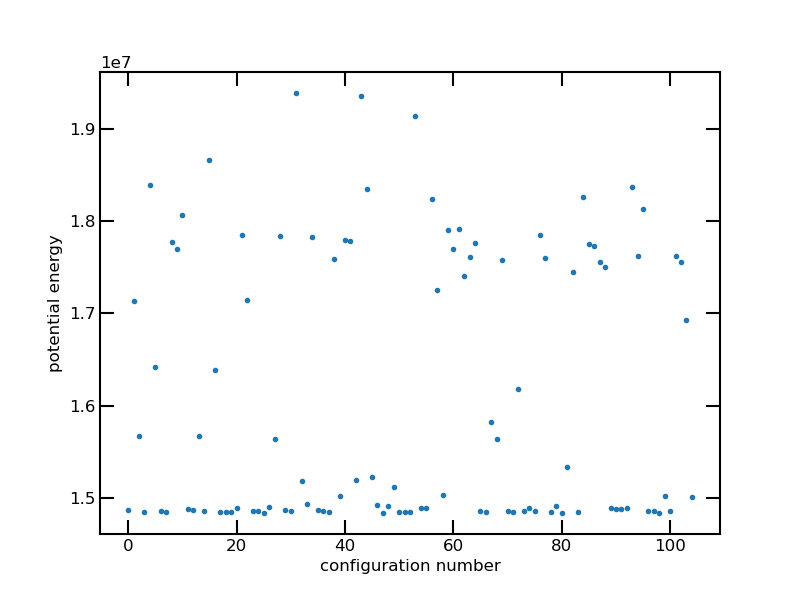
\includegraphics[width=\figwidth]{potential_energy_cell1_1.png}
  \caption{Potential energies for the frames of the first repeat simulation of cell 1.}
  \label{fig:potential_energy_cell1_1}
\end{figure}

\begin{figure}[ht]
\centering
  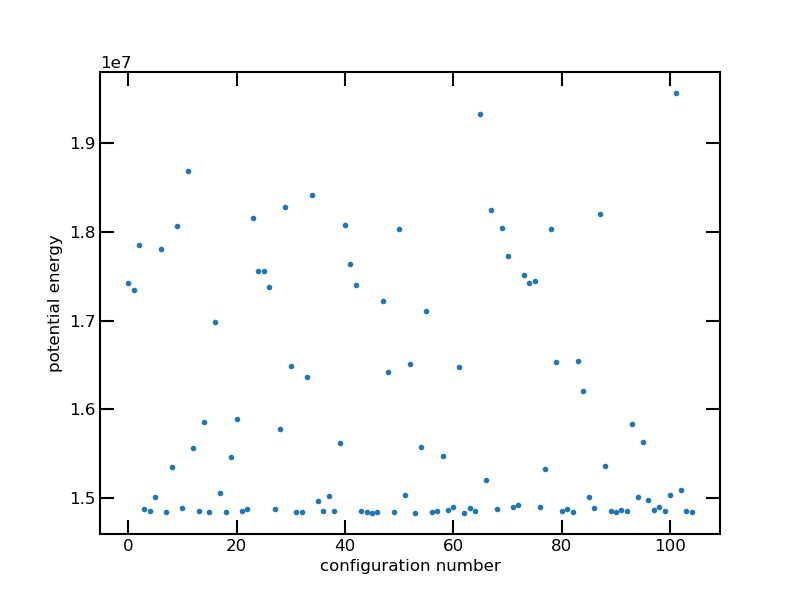
\includegraphics[width=\figwidth]{potential_energy_cell1_2.png}
  \caption{Potential energies for the frames of the second repeat simulation of cell 1.}
  \label{fig:potential_energy_cell1_2}
\end{figure}

\begin{figure}[ht]
\centering
  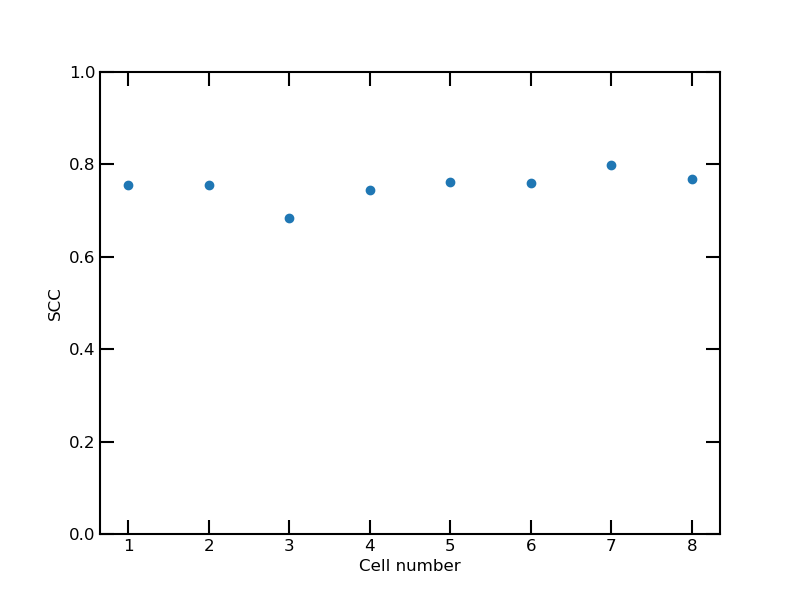
\includegraphics[width=\figwidth]{hic_vs_sim_scc.png}
  \caption{SCCs between the original Hi-C contact matrices and the contact matrices of the simulated cell genomes.}
  \label{fig:hic_vs_sim_scc}
\end{figure}

\begin{figure}[ht]
\centering
  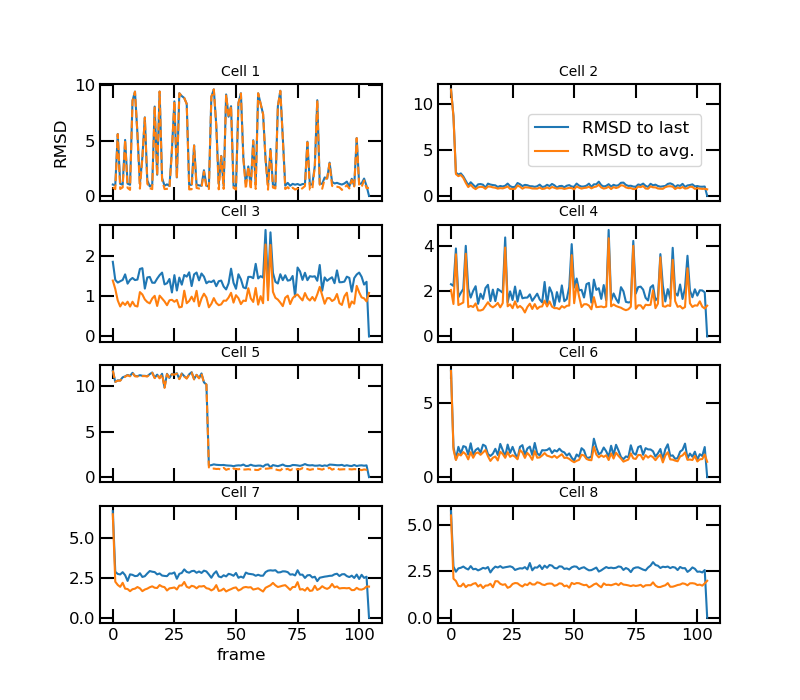
\includegraphics[width=\textwidth+0.5cm]{rmsd_last_vs_avg.png}
  \caption{\textcolor{red}{CAPTION}}
  \label{fig:rmsd_last_vs_avg}
\end{figure}

% chapter tables_and_figures (end)

\chapter{Used Software} % (fold)
\label{cha:used_software}

Figures were created using matplotlib\cite{j_d_hunter_matplotlib_2007} and seaborn\cite{waskom_seaborn_2021}.

\begin{table}[H]
\centering
\label{tab:used_software}
\caption{Software used for simulation and data analysis. Two systems were used, the top one a Manjaro Linux (based on Arch Linux) system and the bottom one a Microsoft Windows system with Anaconda}
  \begin{tabular}{c @{\phantom{abc}} c @{\phantom{abc}} c}
  \toprule
    Package & Version & Package Source \\
  \midrule
    HOOMD-blue & 1.9.7 & built from source \\
    numpy & 1.22.2 & arch repo \\
    scipy & 1.8.0 & arch repo \\
    pandas & 1.4.0 & arch repo \\
    matplotlib & 3.5.1 & arch repo \\
    gsd & 2.5.1 & pip \\
    vmd & 1.9.3 & \url{https://www.ks.uiuc.edu/Research/vmd/} \\
  \midrule
    numpy & 1.20.3 & anaconda \\
    scipy & 1.7.1 & anaconda \\
    pandas & 1.3.4 & anaconda \\
    matplotlib & 3.4.3 & anaconda \\
    gsd & 2.5.1 & pip \\
    hicreppy & 771cf72 & github \\
  \bottomrule
  \end{tabular}
\end{table}

\todo{packages and versions for linux system}


% chapter used_software (end)


\chapter{Renderings of Simuated Cells} % (fold)
\label{cha:renderings_of_simuated_cells}

\newcommand{\cellrenderingwidth}{8cm}
\newcommand{\cellrenderingheight}{8cm}

All renderings rendered using VMD\cite{humphrey_vmd_1996} and tachyon\cite{stone_em_1998} (internal). Colorscale is BGR (from blue at the beginning of the trajectory over green in the middle to red at the end of the trajectory).

\begin{figure}[H]
\centering
  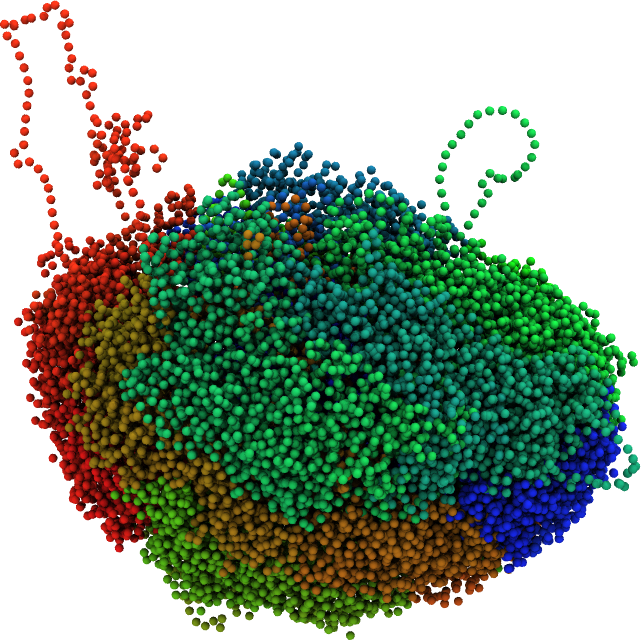
\includegraphics[height=\cellrenderingheight]{cell1_frame104_scene1.png}
  \caption{Cell 1, frame 104, scene 1}
  \label{img:cell1_frame104_scene1}
\end{figure}

\begin{figure}[H]
\centering
  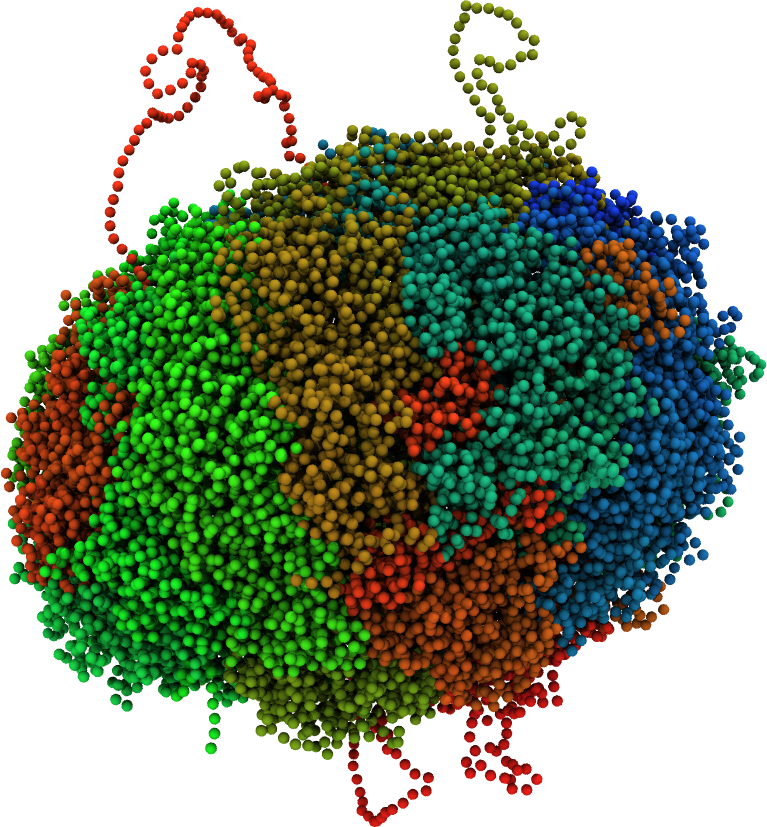
\includegraphics[height=\cellrenderingheight]{cell2_frame104_scene1.png}
  \caption{Cell 2, frame 104, scene 1}
  \label{img:cell2_frame104_scene1}
\end{figure}

\begin{figure}[H]
\centering
  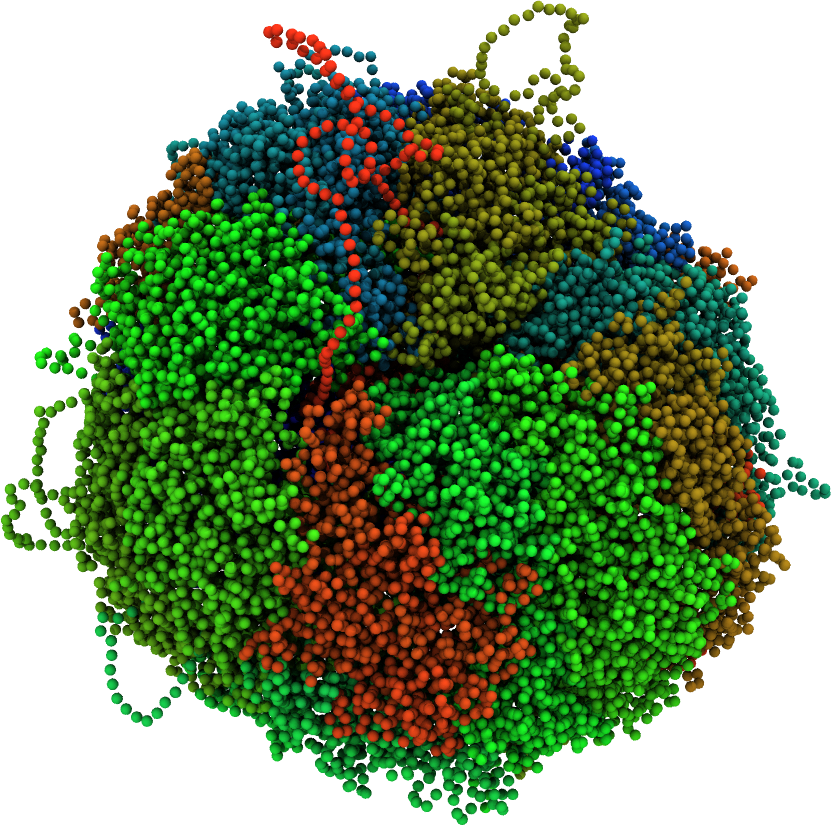
\includegraphics[height=\cellrenderingheight]{cell2_frame104_scene2.png}
  \caption{Cell 2, frame 104, scene 2}
  \label{img:cell2_frame104_scene2}
\end{figure}

\begin{figure}[H]
\centering
  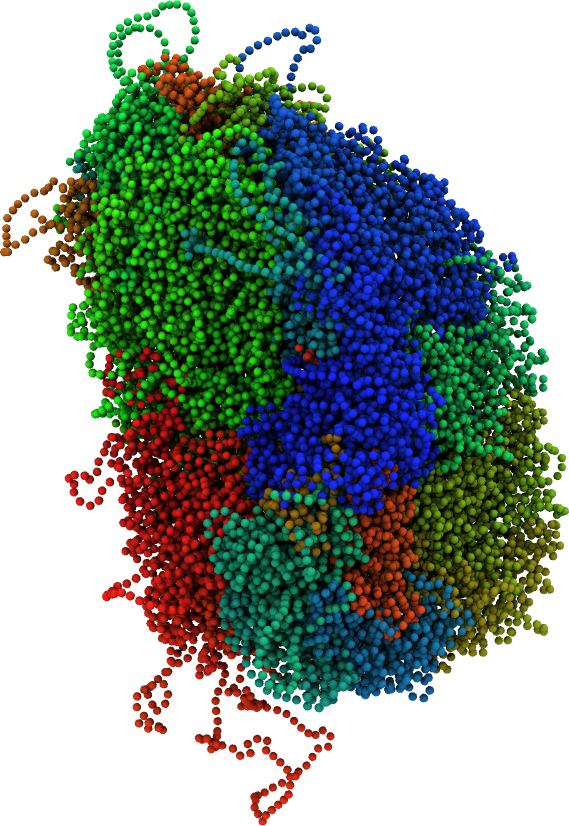
\includegraphics[height=\cellrenderingheight]{cell3_frame104_scene1.png}
  \caption{Cell 3, frame 104, scene 1}
  \label{img:cell3_frame104_scene1}
\end{figure}

\begin{figure}[H]
\centering
  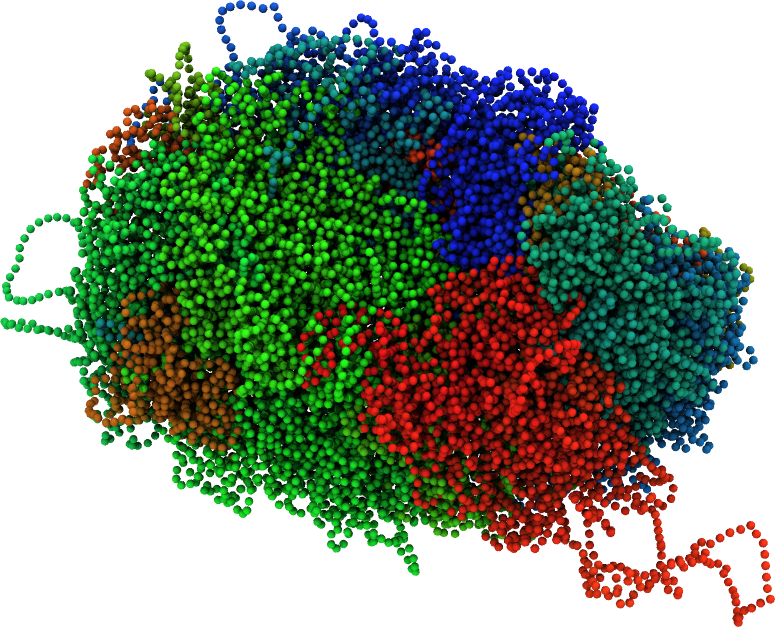
\includegraphics[height=\cellrenderingheight]{cell3_frame104_scene4.png}
  \caption{Cell 3, frame 104, scene 4}
  \label{img:cell3_frame104_scene4}
\end{figure}

\begin{figure}[H]
\centering
  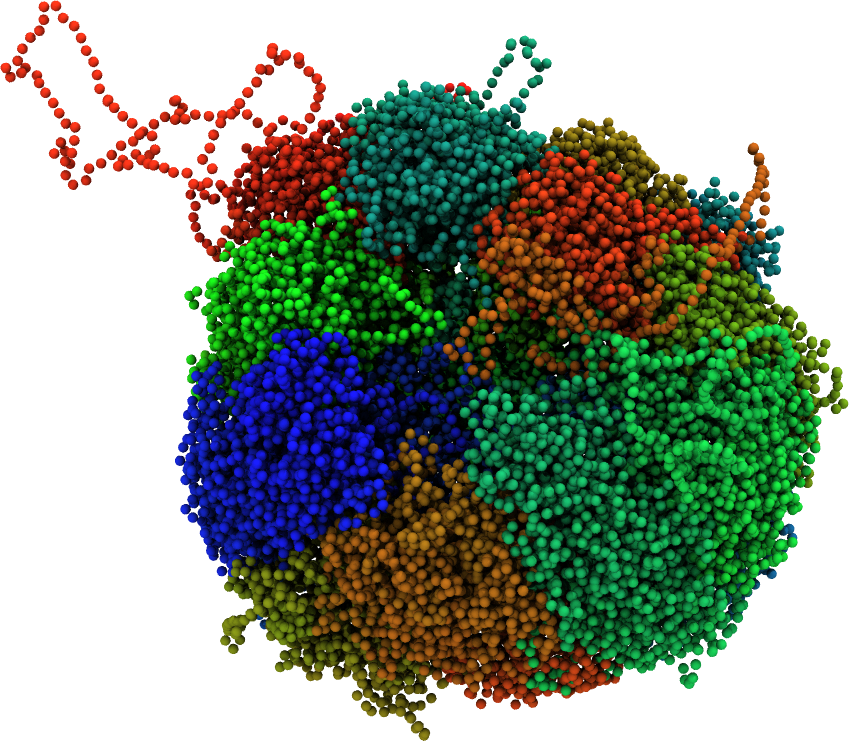
\includegraphics[height=\cellrenderingheight]{cell4_frame104_scene1.png}
  \caption{Cell 4, frame 104, scene 1}
  \label{img:cell4_frame104_scene1}
\end{figure}

\begin{figure}[H]
\centering
  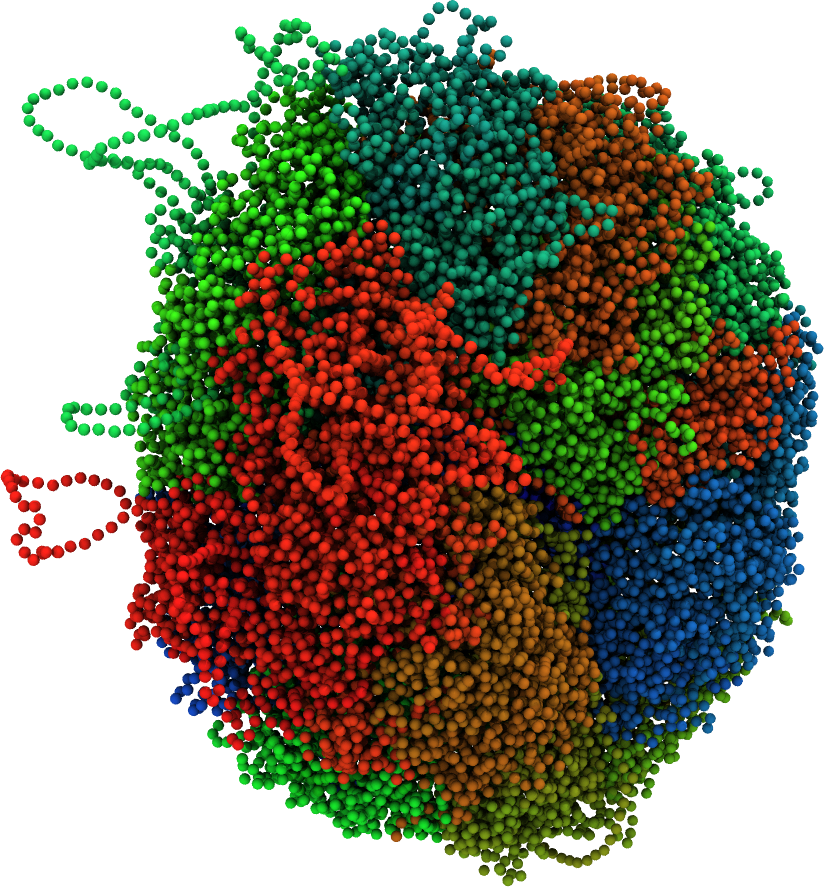
\includegraphics[height=\cellrenderingheight]{cell5_frame036_scene1.png}
  \caption{Cell 5, frame 36, scene 1}
  \label{img:cell5_frame036_scene1}
\end{figure}

\begin{figure}[H]
\centering
  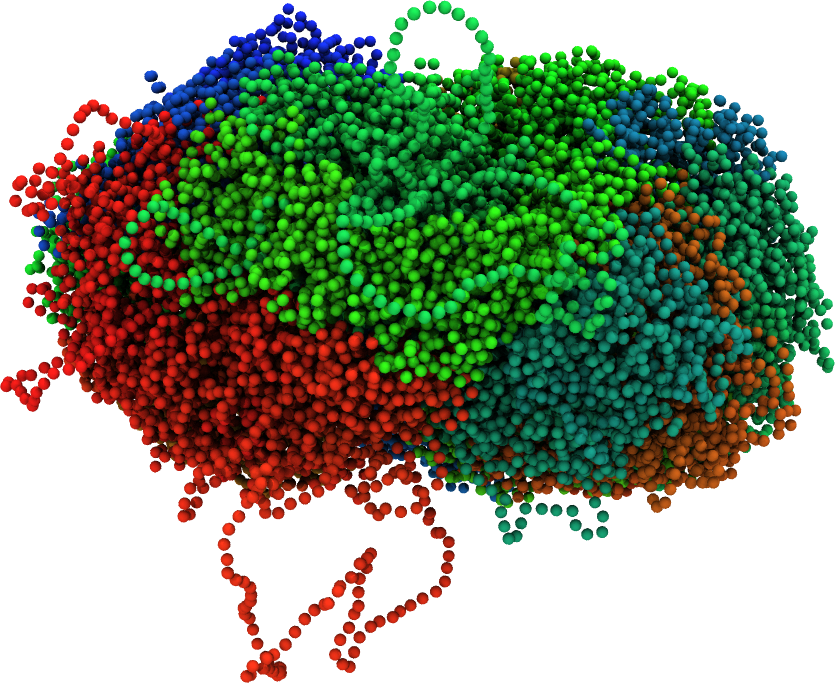
\includegraphics[height=\cellrenderingheight]{cell5_frame036_scene2.png}
  \caption{Cell 5, frame 36, scene 2}
  \label{img:cell5_frame036_scene2}
\end{figure}

\begin{figure}[H]
\centering
  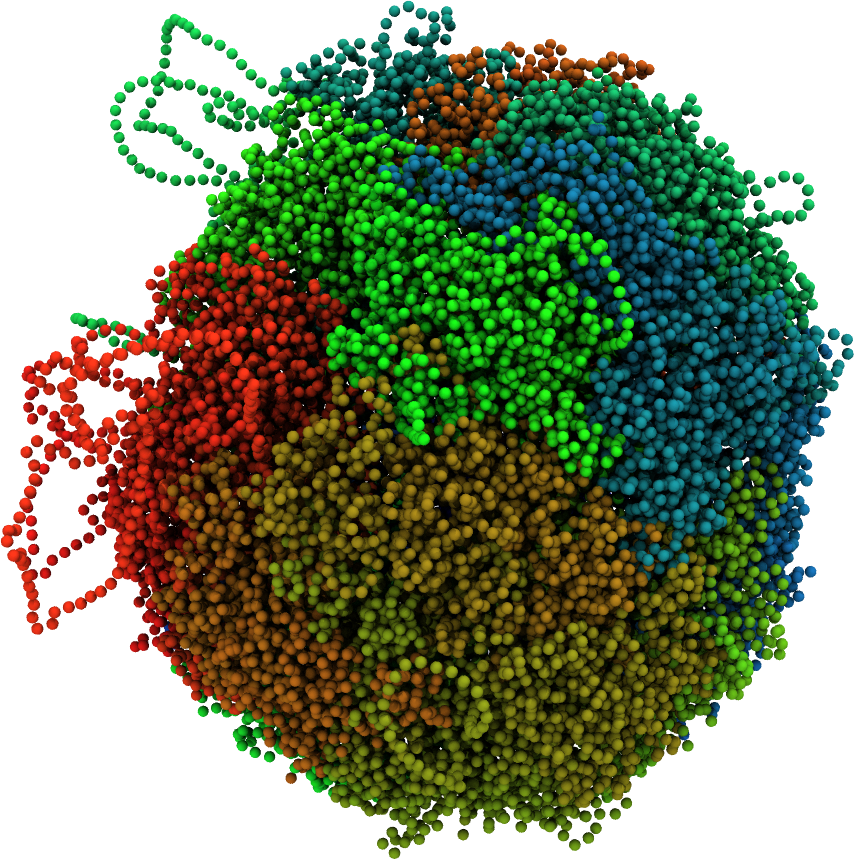
\includegraphics[height=\cellrenderingheight]{cell5_frame104_scene1.png}
  \caption{Cell 5, frame 104, scene 1}
  \label{img:cell5_frame104_scene1}
\end{figure}

\begin{figure}[H]
\centering
  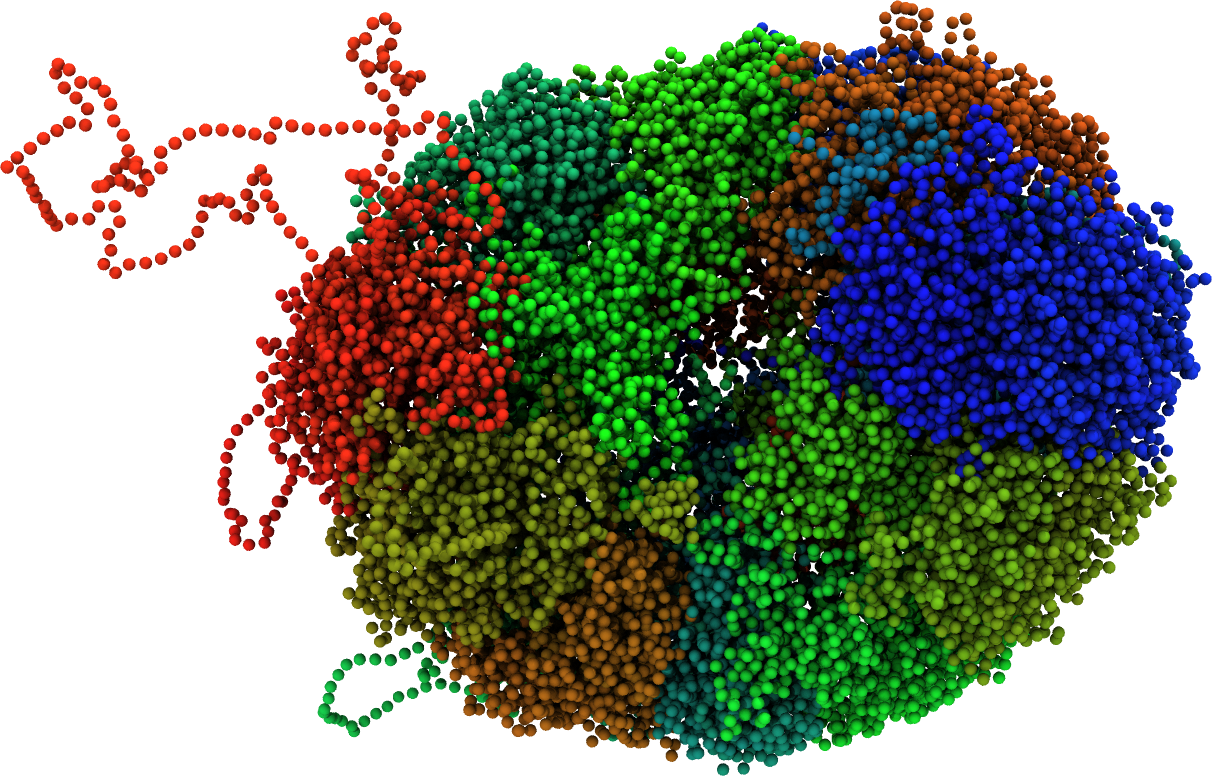
\includegraphics[height=\cellrenderingheight]{cell6_frame104_scene1.png}
  \caption{Cell 6, frame 104, scene 1}
  \label{img:cell6_frame104_scene1}
\end{figure}

\begin{figure}[H]
\centering
  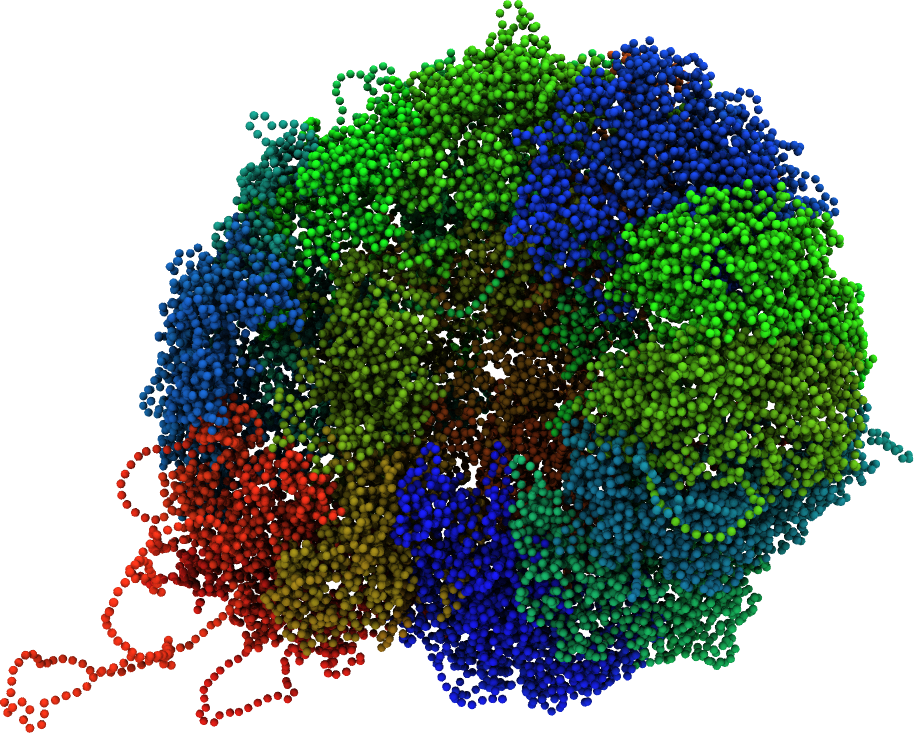
\includegraphics[height=\cellrenderingheight]{cell7_frame104_scene1.png}
  \caption{Cell 7, frame 104, scene 1}
  \label{img:cell7_frame104_scene1}
\end{figure}

\begin{figure}[H]
\centering
  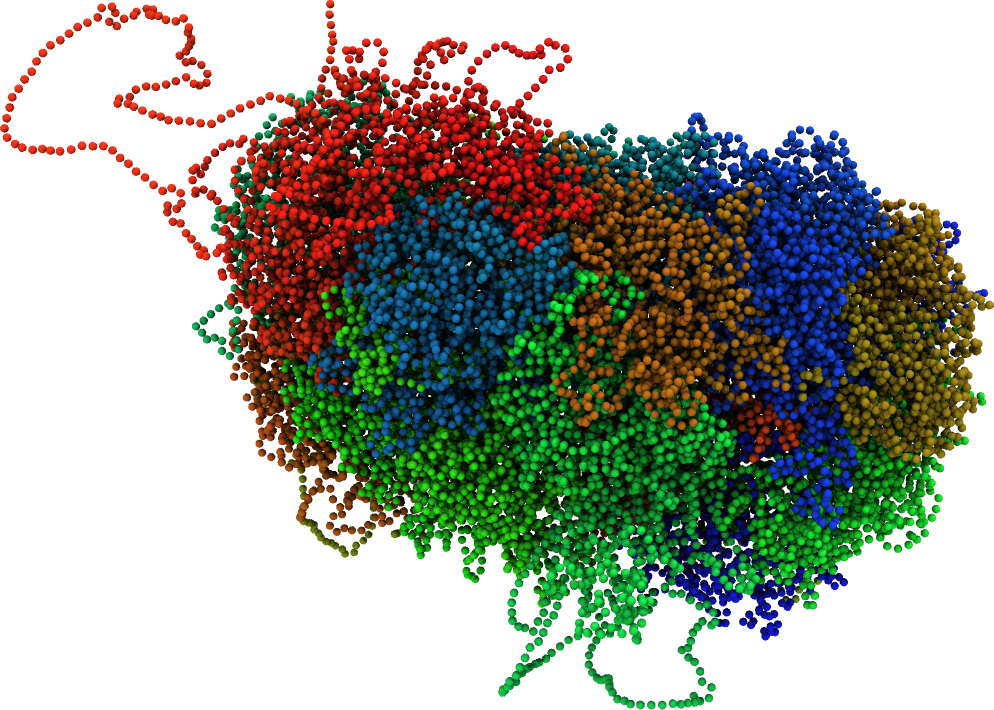
\includegraphics[height=\cellrenderingheight]{cell8_frame104_scene2.png}
  \caption{Cell 8, frame 104, scene 2}
  \label{img:cell8_frame104_scene2}
\end{figure}


% chapter renderings_of_simuated_cells (end)

%_______________________________________________________________________________
% \chapter{Weiterführende Details zur Arbeit} % (fold)
% \label{cha:weiterführende_details_zur_arbeit}

% Manch wichtiger Teil Ihrer tatsächlichen Arbeit ist zu technisch 
% und würde den Hauptteil des Textes unübersichtlich machen, 
% beispielsweise wenn es um die Details des Versuchsaufbaus in einer 
% experimentellen Arbeit oder um den für eine numerische Auswertung 
% verwendeten Algorithmus geht. Dennoch ist es sinnvoll, entsprechende 
% Beschreibungen in einem Anhang Ihrer Bachelorarbeit aufzunehmen. 
% Insbesondere für zukünftige Arbeiten, die an Ihre Bachelorarbeit 
% anschließen, sind dies manchmal hilfreiche Informationen.

% % chapter weiterführende_details_zur_arbeit (end)

%_______________________________________________________________________________
% \chapter{Thanking} % (fold)
% \label{cha:thanking}

% ... an wen auch immer. Denken Sie an Ihre Freundinnen und Freunde, 
% Familie, Lehrer, Berater und Kollegen.

% chapter thanking (end)

%_______________________________________________________________________________
% \chapter{References} % (fold)
% \label{cha:references}

% Machen Sie genaue Angaben, so dass die verwendeten Literaturstellen 
% eindeutig identifiziert und aufgefunden werden können.
% Bei Lehrbüchern cite{Weinberg:1995mt} ist es sinnvoll, 
% den Titel anzugeben, eventuell auch die Ausgabe. Bei Artikeln in 
% Fachzeitschriften cite{Moch:2001zr} ist es üblich, nur die 
% gebräuchlichen Abkürzungen für den Titel der Zeitschrift, Band, 
% Erscheinungsjahr und Seite anzugeben. Unter Umständen kann es auch 
% sinnvoll sein, im Internet aufgefundene Informationsquellen anzugeben, 
% zum Beispiel für Software cite{LoopTools} oder zu den Details von 
% Ergebnissen großer experimenteller Kollaborationen. Es ist 
% selbstverständlich, dass Sie auch Bachelor- cite{BA:Freund}, 
% Diplom- oder Doktorarbeiten angeben, wenn Sie diese in Ihrer eigenen 
% Arbeit verwendet haben.
% \medskip

% Im folgenden Beispiel werden die in der Datei \texttt{h-physrev3.bst} 
% enthaltenen Anweisungen als Stilvorlage verwendet. Andere 
% Möglichkeiten für die Gestaltung eines Literaturverzeichnisses 
% findet man im Internet: \url{http://janeden.net/bibliographien-mit-latex}.

% \renewcommand{\bibname}{Literaturverzeichnis} 
% \bibliographystyle{h-physrev3}
% \begin{thebibliography}{99}

% %\cite{thepnews}
% \bibitem{EbelBliefert}
% H.\ F.\ Ebel, C.\ Bliefert, 
%   ``Bachelor-, Master- und Doktorarbeit: Anleitungen für den 
%   naturwissenschaftlich-technischen Nachwuchs,''
%   Wiley-VCH, Weinheim (2009). 
% \bibitem{thepnews}
%   S.~Becker, D.~Götz, C.~Reuschle, C.~Schwan, S.~Weinzierl,  
%   \url{http://wwwthep.physik.uni-mainz.de/site/news/168/}.

% %\cite{Weinberg:1995mt}
% \bibitem{Weinberg:1995mt}
%   S.~Weinberg,
%   ``The Quantum theory of fields. Vol. 1: Foundations,''
%   Cambridge, UK: Univ. Pr. (1995) 609 p.

% %\cite{Moch:2001zr}
% \bibitem{Moch:2001zr}
%   S.~Moch, P.~Uwer, S.~Weinzierl,
%   %``Nested sums, expansion of transcendental functions and multiscale 
%   % multiloop integrals,''
%   J.\ Math.\ Phys.\  {43 } (2002)  3363-3386.
%   [hep-ph/0110083].

% %\cite{LoopTools}
% \bibitem{LoopTools}
%   T.~Hahn, 
%   ``The LoopTools Site,''
%   \url{http://www.feynarts.de/looptools/}.

% %\cite{BA:Freund}
% \bibitem{BA:Freund}
%   B.~Freund, 
%   Bachelorarbeit, Johannes Gutenberg-Universität Mainz, 2012.

% \end{thebibliography}

% chapter references (end)


\end{document}